
\input{../../Papers/header.tex}

\newcommand{\fakesection}[1]{%
  \par\refstepcounter{section}% Increase section counter
  \sectionmark{#1}% Add section mark (header)
  \addcontentsline{toc}{section}{Lecture \thesection: #1}% Add section to ToC
  % Add more content here, if needed.
}
\newcommand{\fakesectionb}[1]{%
  \par\refstepcounter{section}% Increase section counter
  \sectionmark{#1}% Add section mark (header)
  \addcontentsline{toc}{section}{\protect#1}% Add section to ToC
  % Add more content here, if needed.
}
\usepackage{pdfpages}
\usepackage{hyperref}

\title{Econometric Methods}
\author{Gary Chamberlain}
\date{}  
\begin{document}
\maketitle

This document contains the set of lecture notes from the late Gary
Chamberlain's 2010 Econometrics class (EC2120) that I (Paul
Goldsmith-Pinkham) took during my economics Ph.D. at Harvard
University. Gary was a remarkable teacher and this class was an
amazing experience for me as a young economist.

A few things worth noting from my experience taking this course: 
\begin{itemize}
\item The course is somewhat unique in not introducing any inference
  until Lecture 7 (halfway through the course). The focus prior to
  this is exclusively on estimation using regression.
\item The lectures are linked together in groups (even though they are
  not marked this way). Lectures 1-3 reflect the underlying setup in
  notation and framework for the rest of the course. Lectures 6-9
  setup inference. Lecture 9-11 discuss a general framework for using
  moment conditions.
\item During my semester, we never got through lectures 13-15, which
  suggests that this is a lot of material for a single semester.
\item Gary would continually refer back to Lecture 4 and Lecture 9
  (indeed, I have Gary's voice saying ``if we think back to the Note 9
  framework...'' burned into my brain. As a result, these are also
  some of the longest and densest lectures.
\item The last 4 sections are review problems that Gary provided for
  preparation for the final exam. These are very fun problems, but we
  were not provided solutions. So, you'll have to figure them out on
  your own!
\end{itemize}

- Paul Goldsmith-Pinkham (Harvard Ph.D., 2015)

\clearpage

\tableofcontents

\clearpage

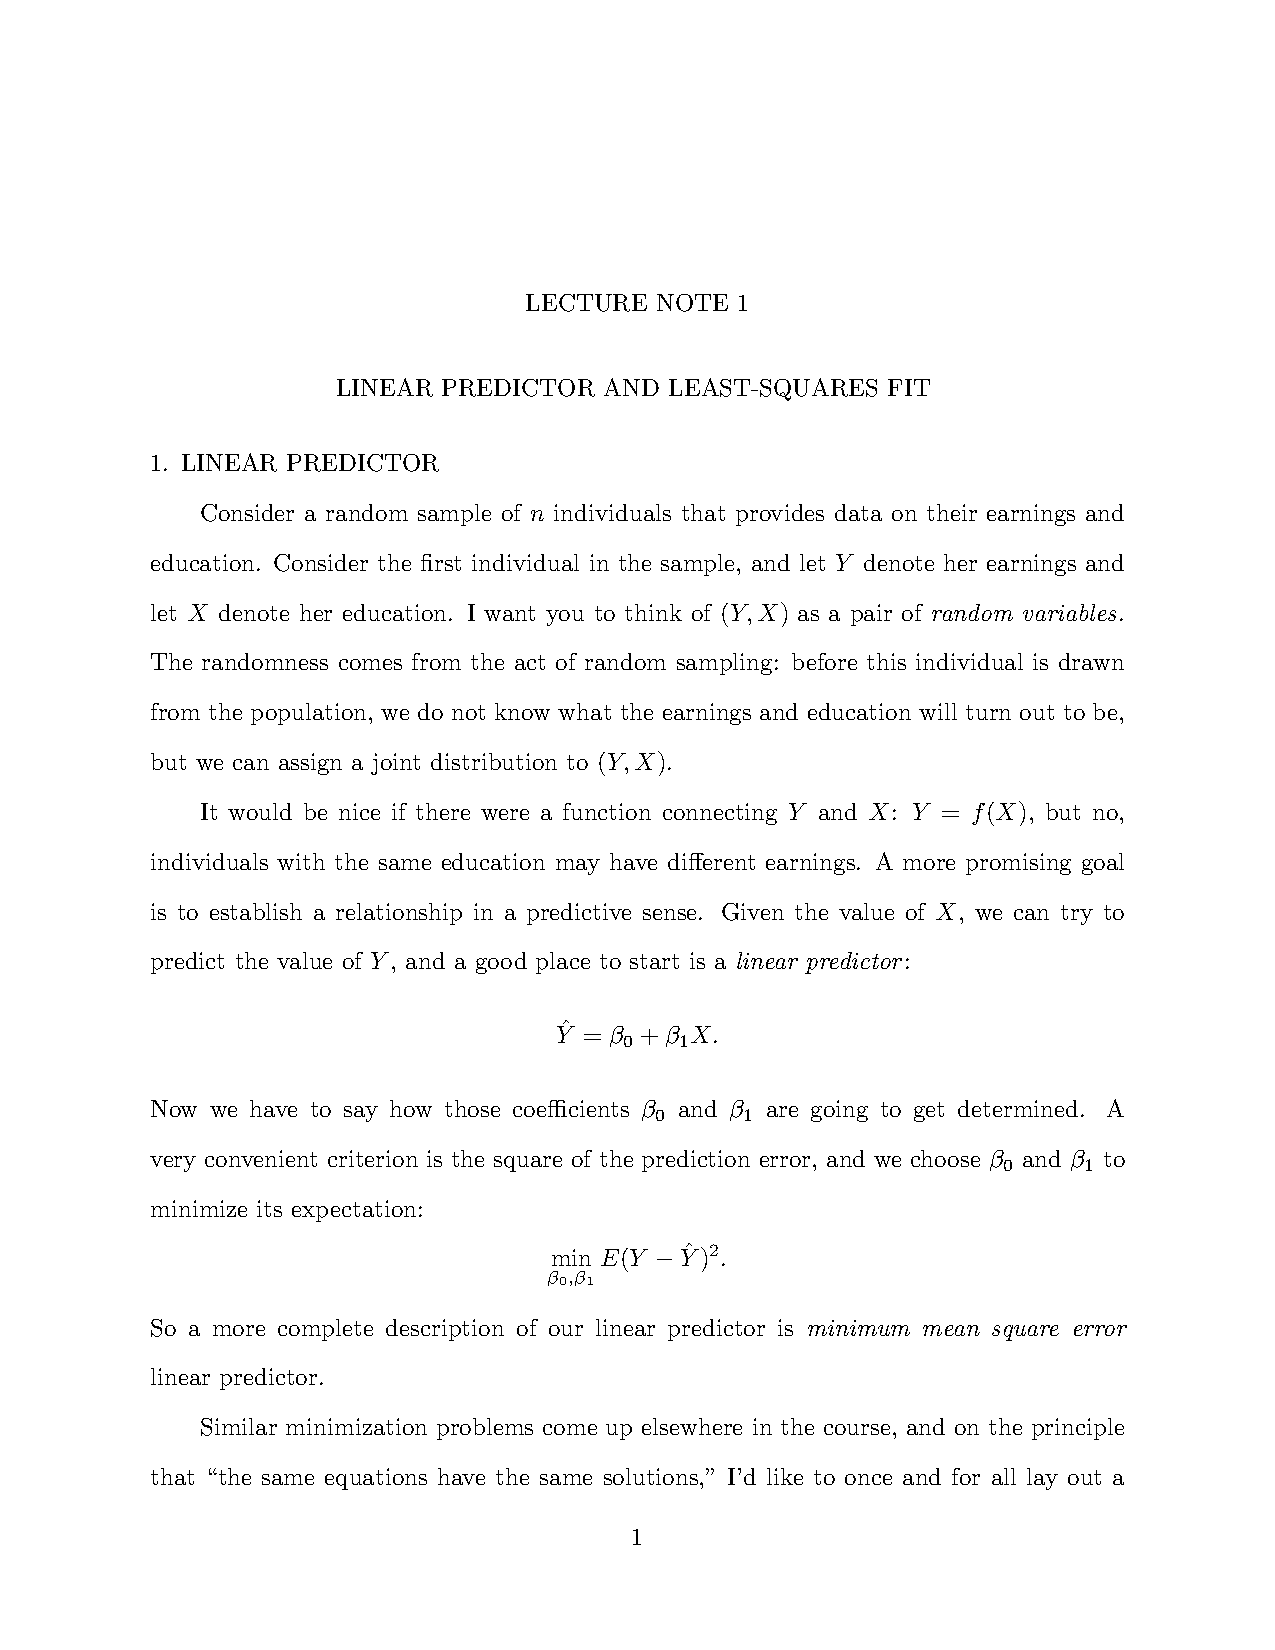
\includepdf[pages=1,pagecommand={\fakesection{Linear Predictor and Least-Squares Fit}\label{lecture1}},linktodoc=true, clip,trim=0mm 22mm 0mm 24mm]{Lecture_Note_1_edit.pdf}
\includepdf[pages=2-,pagecommand={}, clip,trim=0mm 22mm 0mm 24mm]{Lecture_Note_1_edit.pdf}
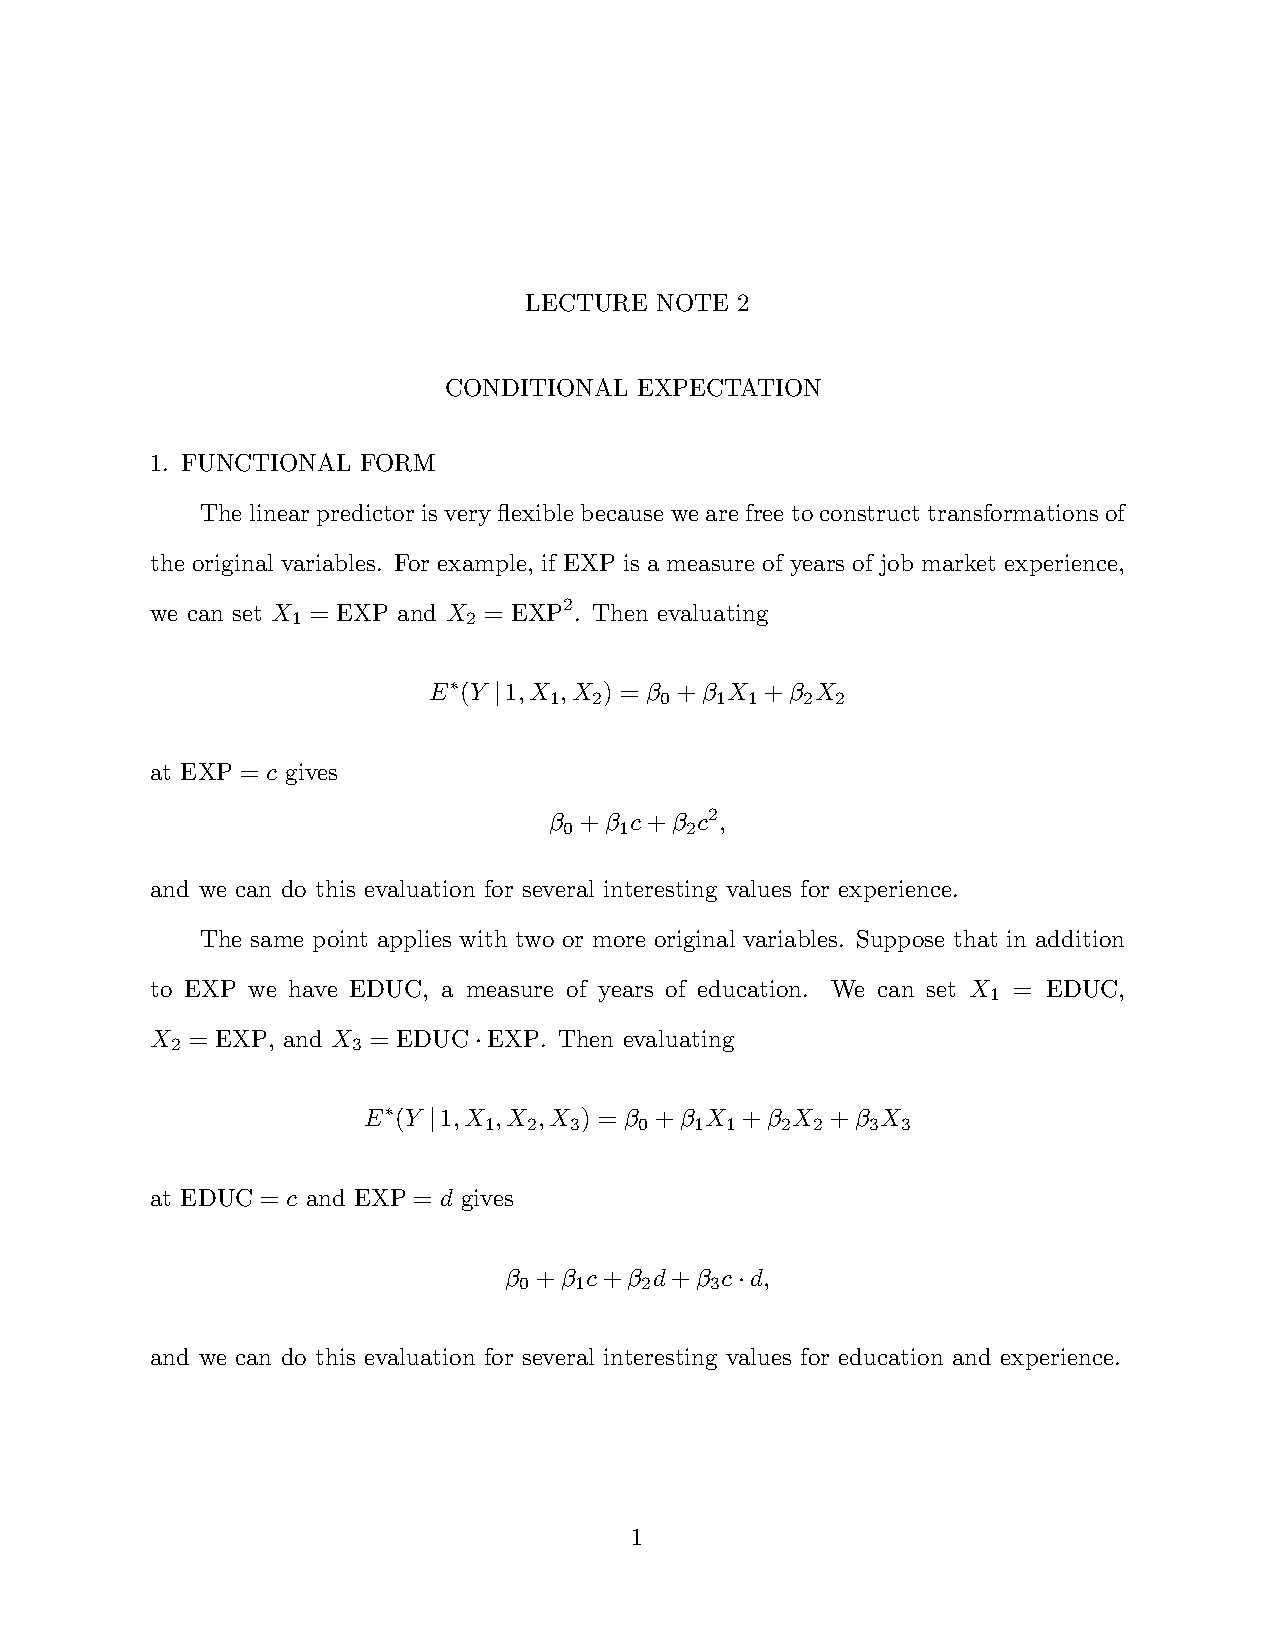
\includepdf[pages=1, pagecommand={\fakesection{Conditional Expectation}\label{lecture2}},linktodoc=true,clip,trim=0mm 22mm 0mm 24mm]{Lecture_Note_2_edit.pdf}
\includepdf[pages=2-,pagecommand={},clip,trim=0mm 22mm 0mm 24mm]{Lecture_Note_2.pdf}
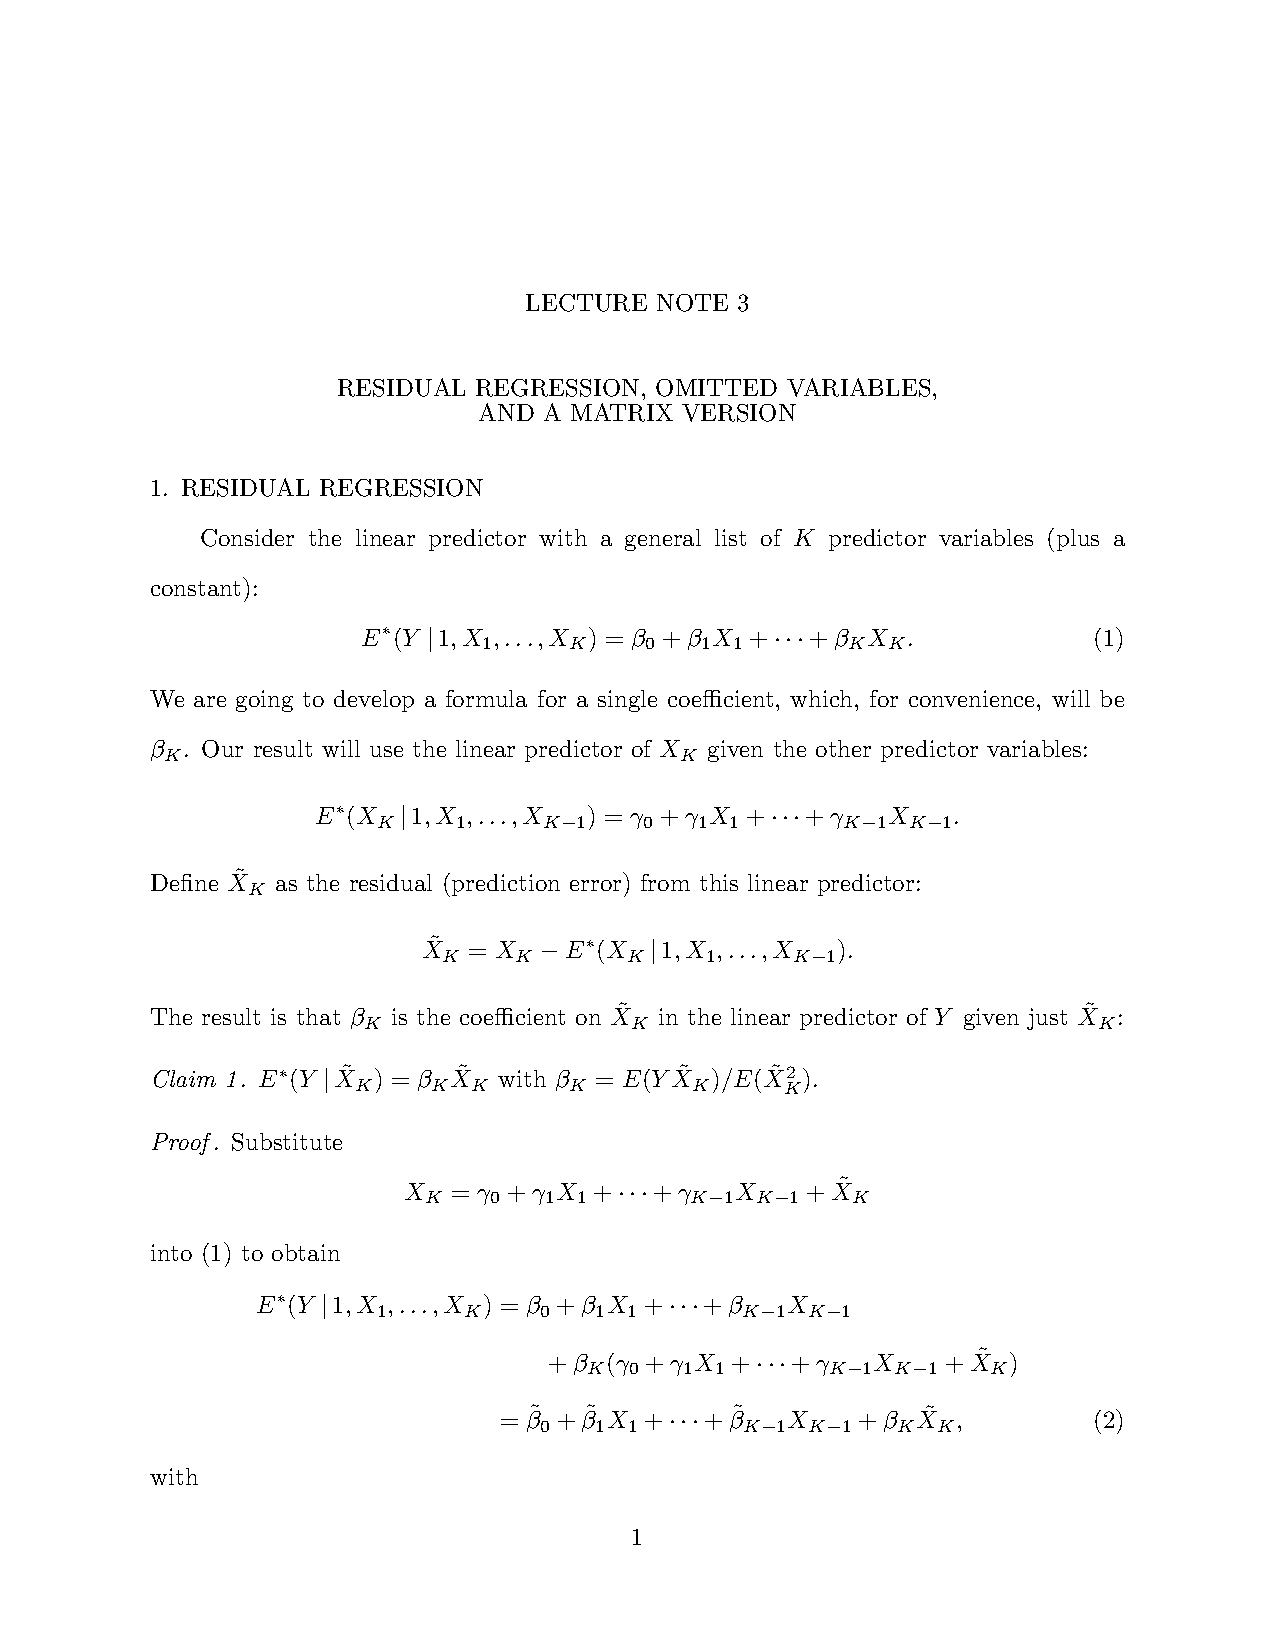
\includepdf[pages=1, pagecommand={\fakesection{Residual Regression, Omitted Variables, and a Matrix Version}\label{lecture3}},linktodoc=true,clip,trim=0mm 22mm 0mm 24mm]{Lecture_Note_3.pdf}
\includepdf[pages=2-,pagecommand={},clip,trim=0mm 22mm 0mm 24mm]{Lecture_Note_3.pdf}
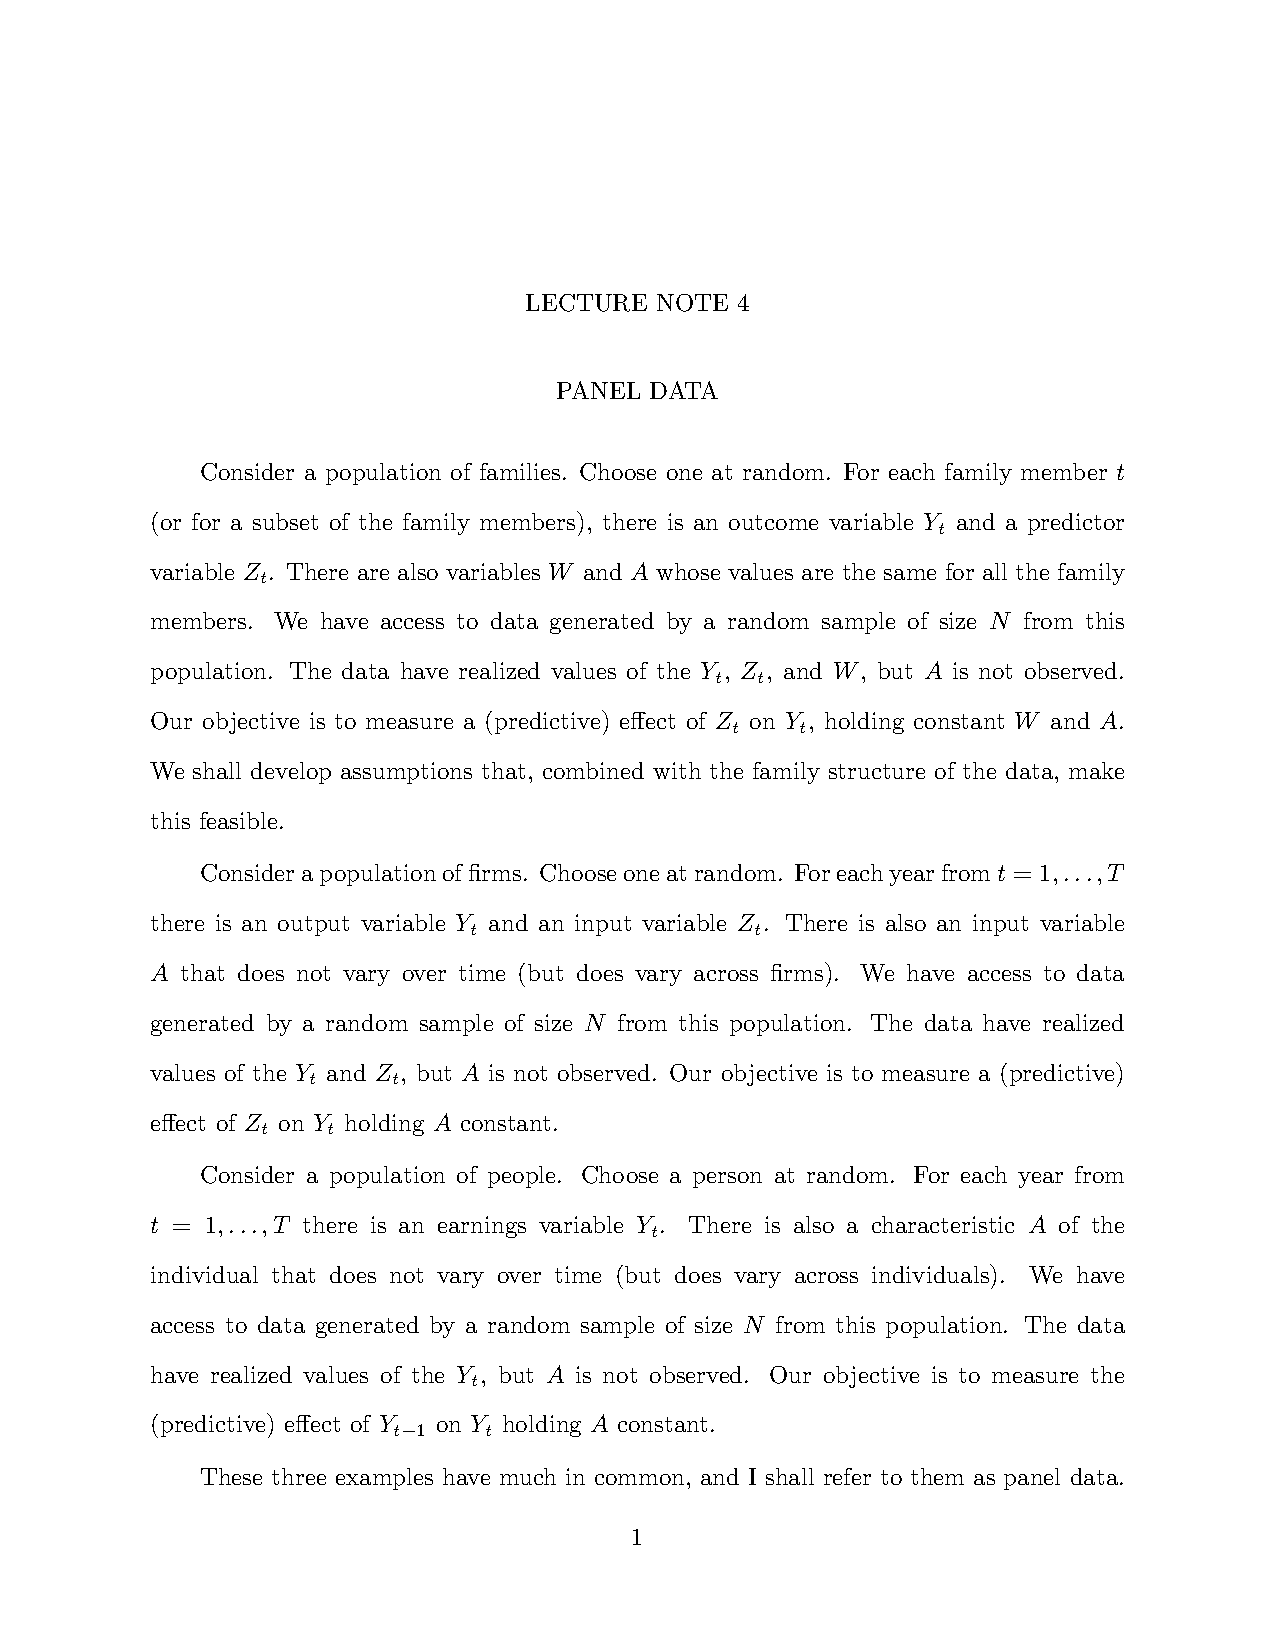
\includepdf[pages=1, pagecommand={\fakesection{Panel Data}\label{lecture4}},linktodoc=true,clip,trim=0mm 22mm 0mm 24mm]{Lecture_Note_4.pdf}
\includepdf[pages=2-,pagecommand={},clip,trim=0mm 22mm 0mm 24mm]{Lecture_Note_4.pdf}
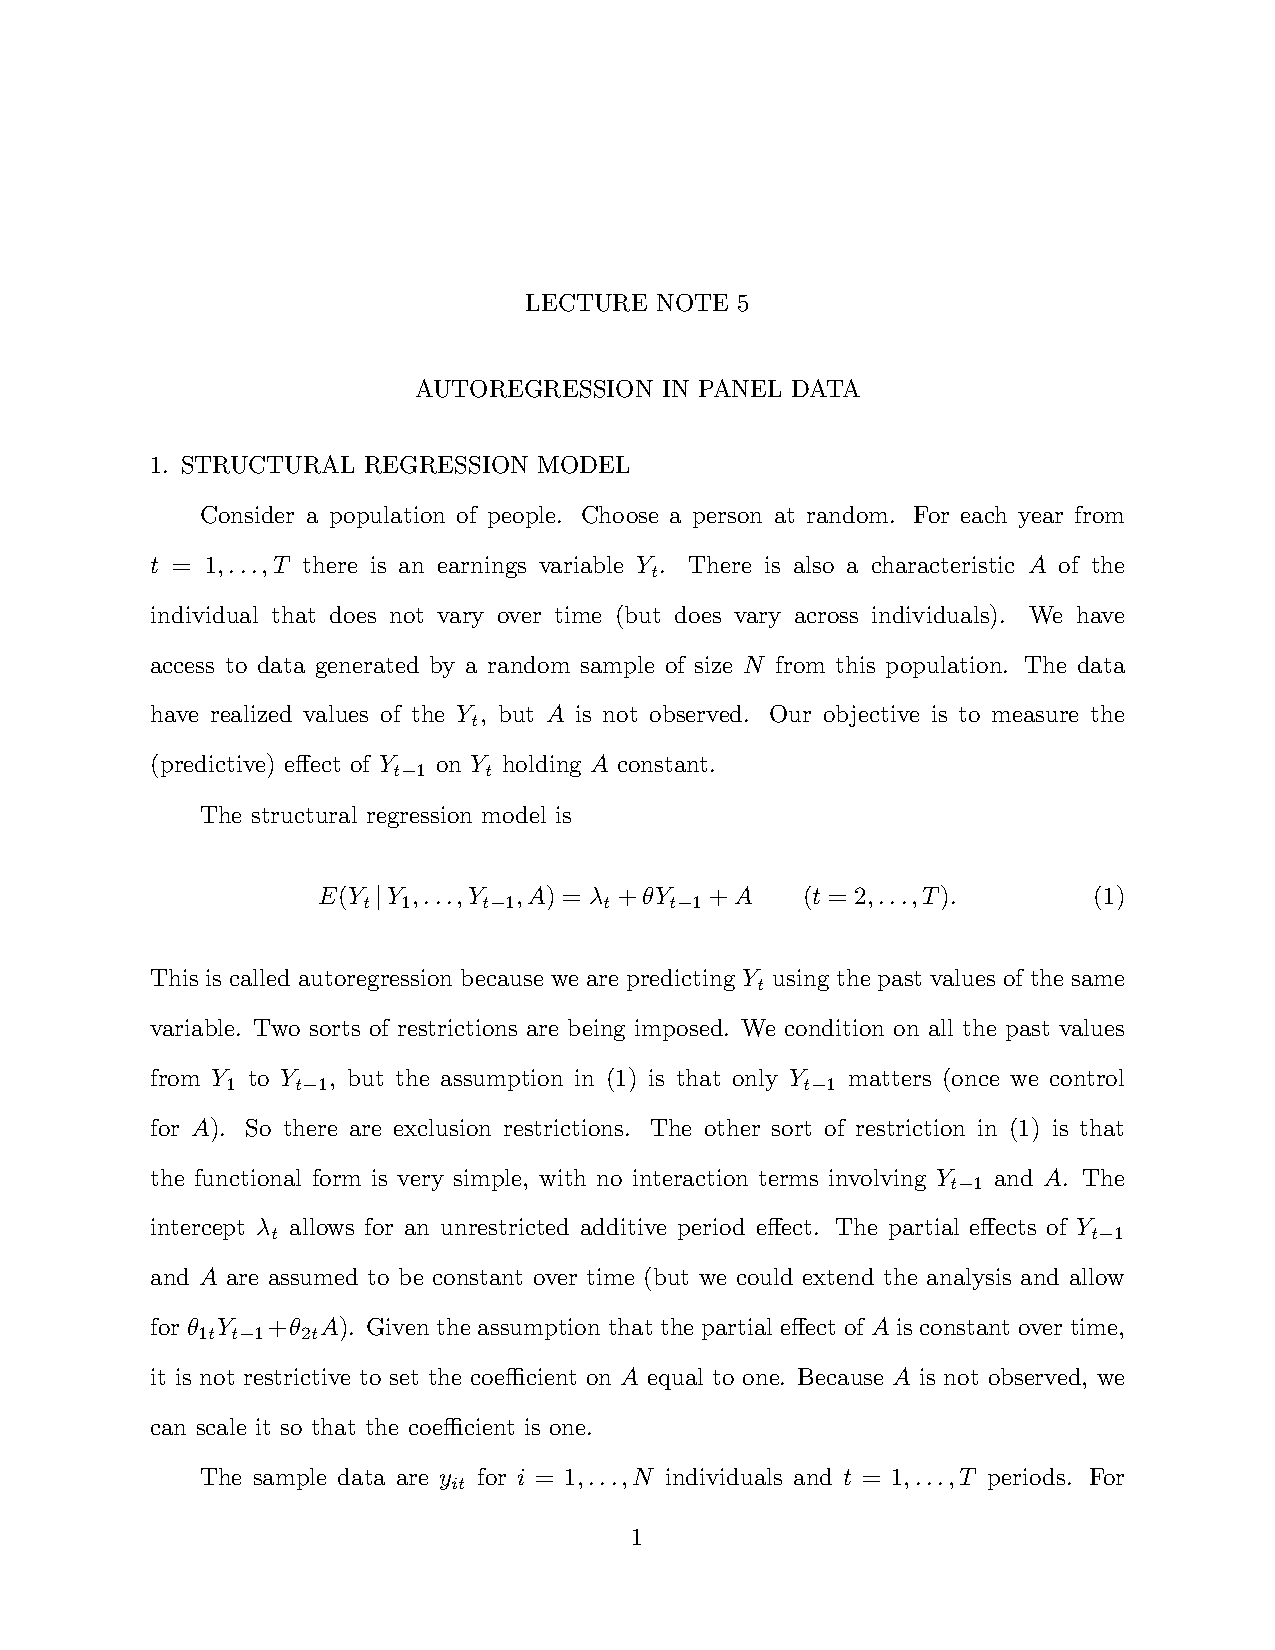
\includepdf[pages=1, pagecommand={\fakesection{Autoregression in Panel Data}\label{lecture5}},linktodoc=true,clip,trim=0mm 22mm 0mm 24mm]{Lecture_Note_5.pdf}
\includepdf[pages=2-,pagecommand={},clip,trim=0mm 22mm 0mm 24mm]{Lecture_Note_5.pdf}
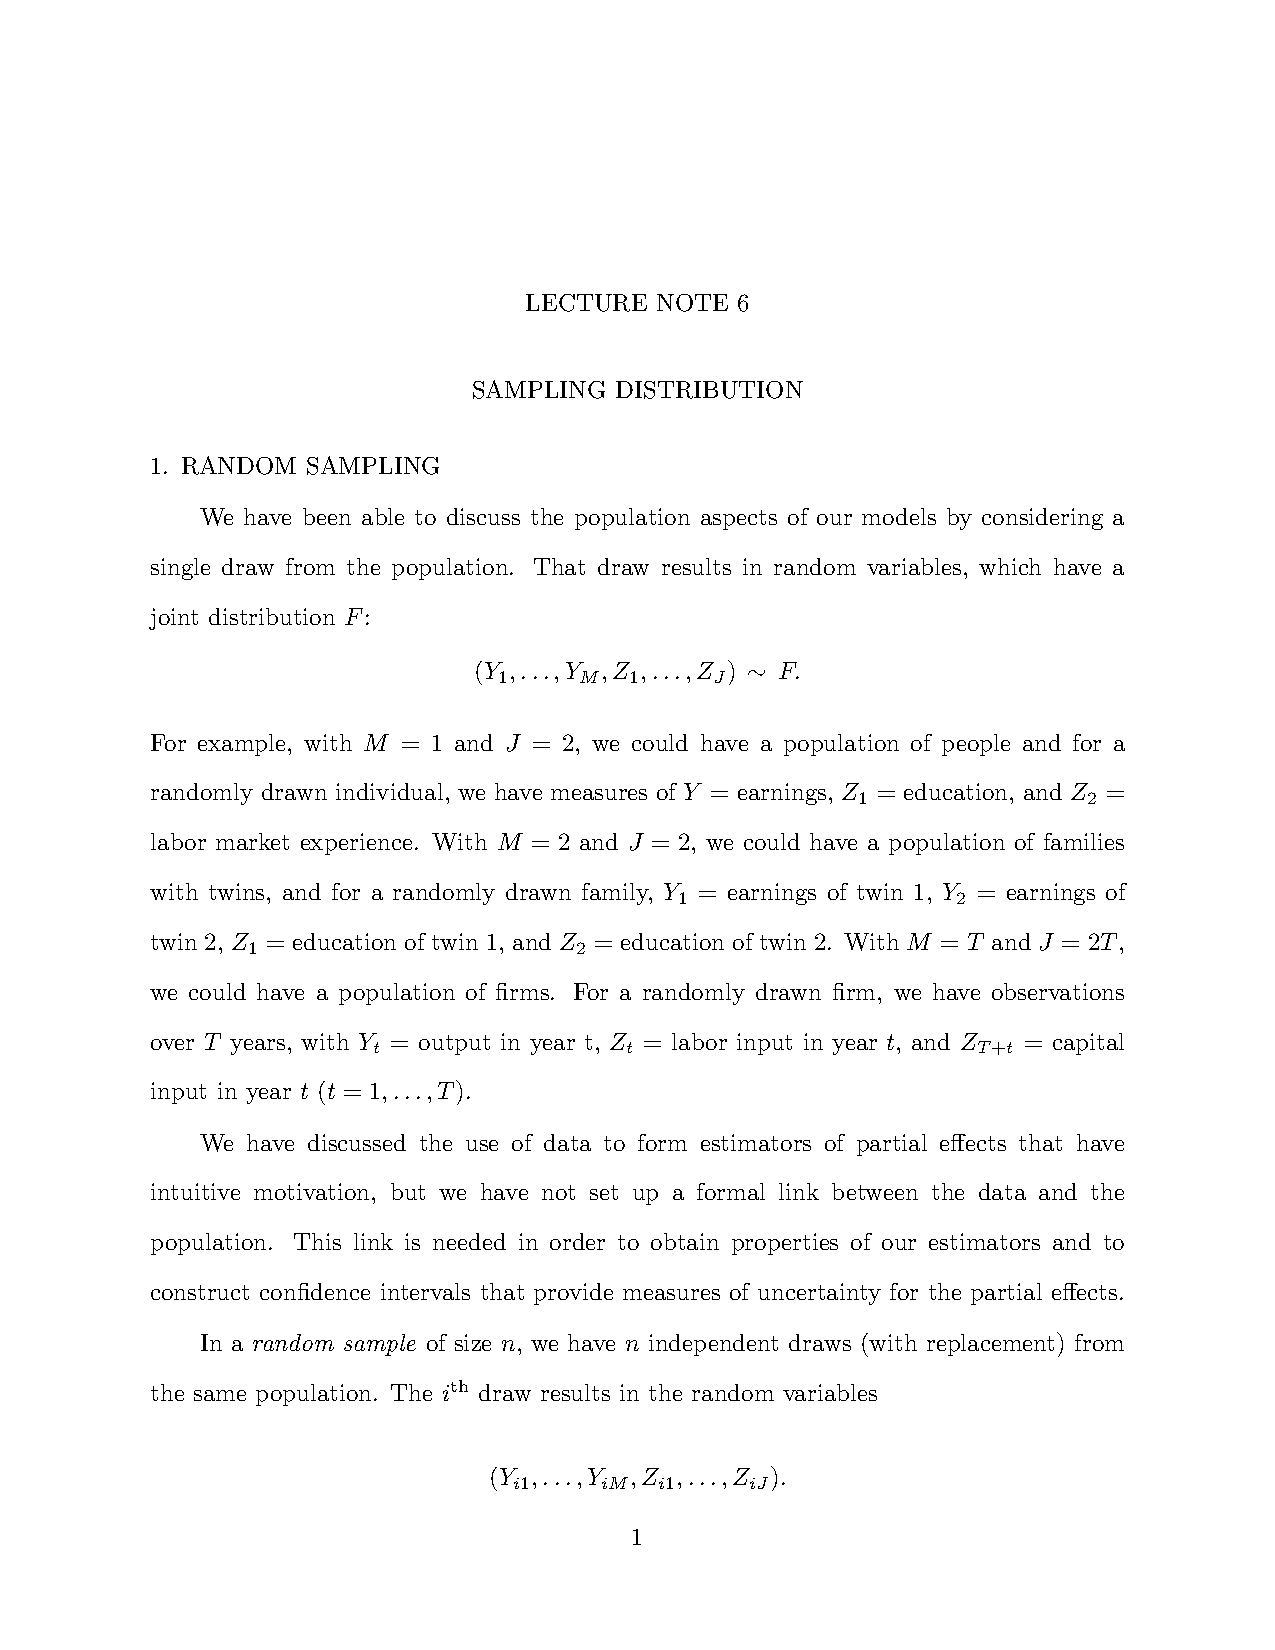
\includepdf[pages=1, pagecommand={\fakesection{Sampling Distribution}\label{lecture6}},linktodoc=true,clip,trim=0mm 22mm 0mm 24mm]{Lecture_Note_6.pdf}
\includepdf[pages=2-,pagecommand={},clip,trim=0mm 22mm 0mm 24mm]{Lecture_Note_6.pdf}
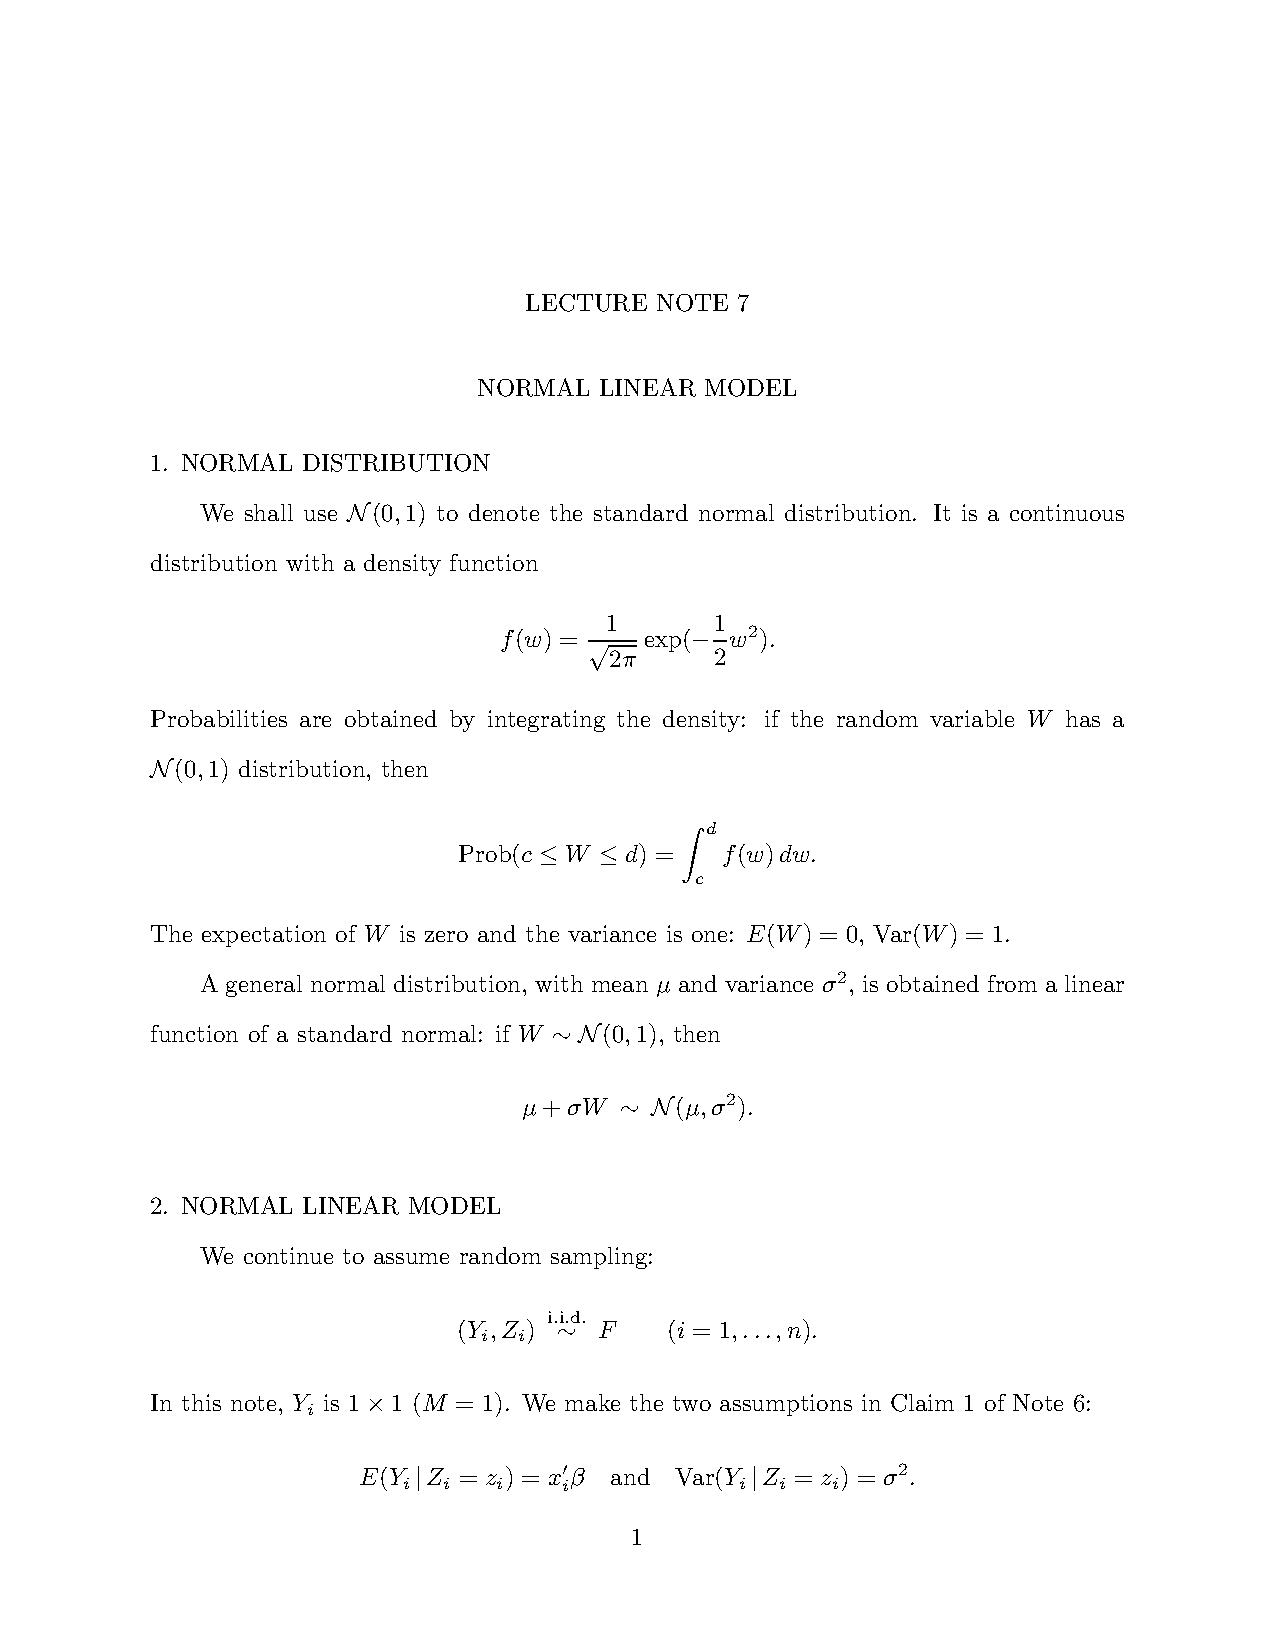
\includepdf[pages=1, pagecommand={\fakesection{Normal Linear Model}\label{lecture7}},linktodoc=true,clip,trim=0mm 22mm 0mm 24mm]{Lecture_Note_7.pdf}
\includepdf[pages=2-,pagecommand={},clip,trim=0mm 22mm 0mm 24mm]{Lecture_Note_7.pdf}
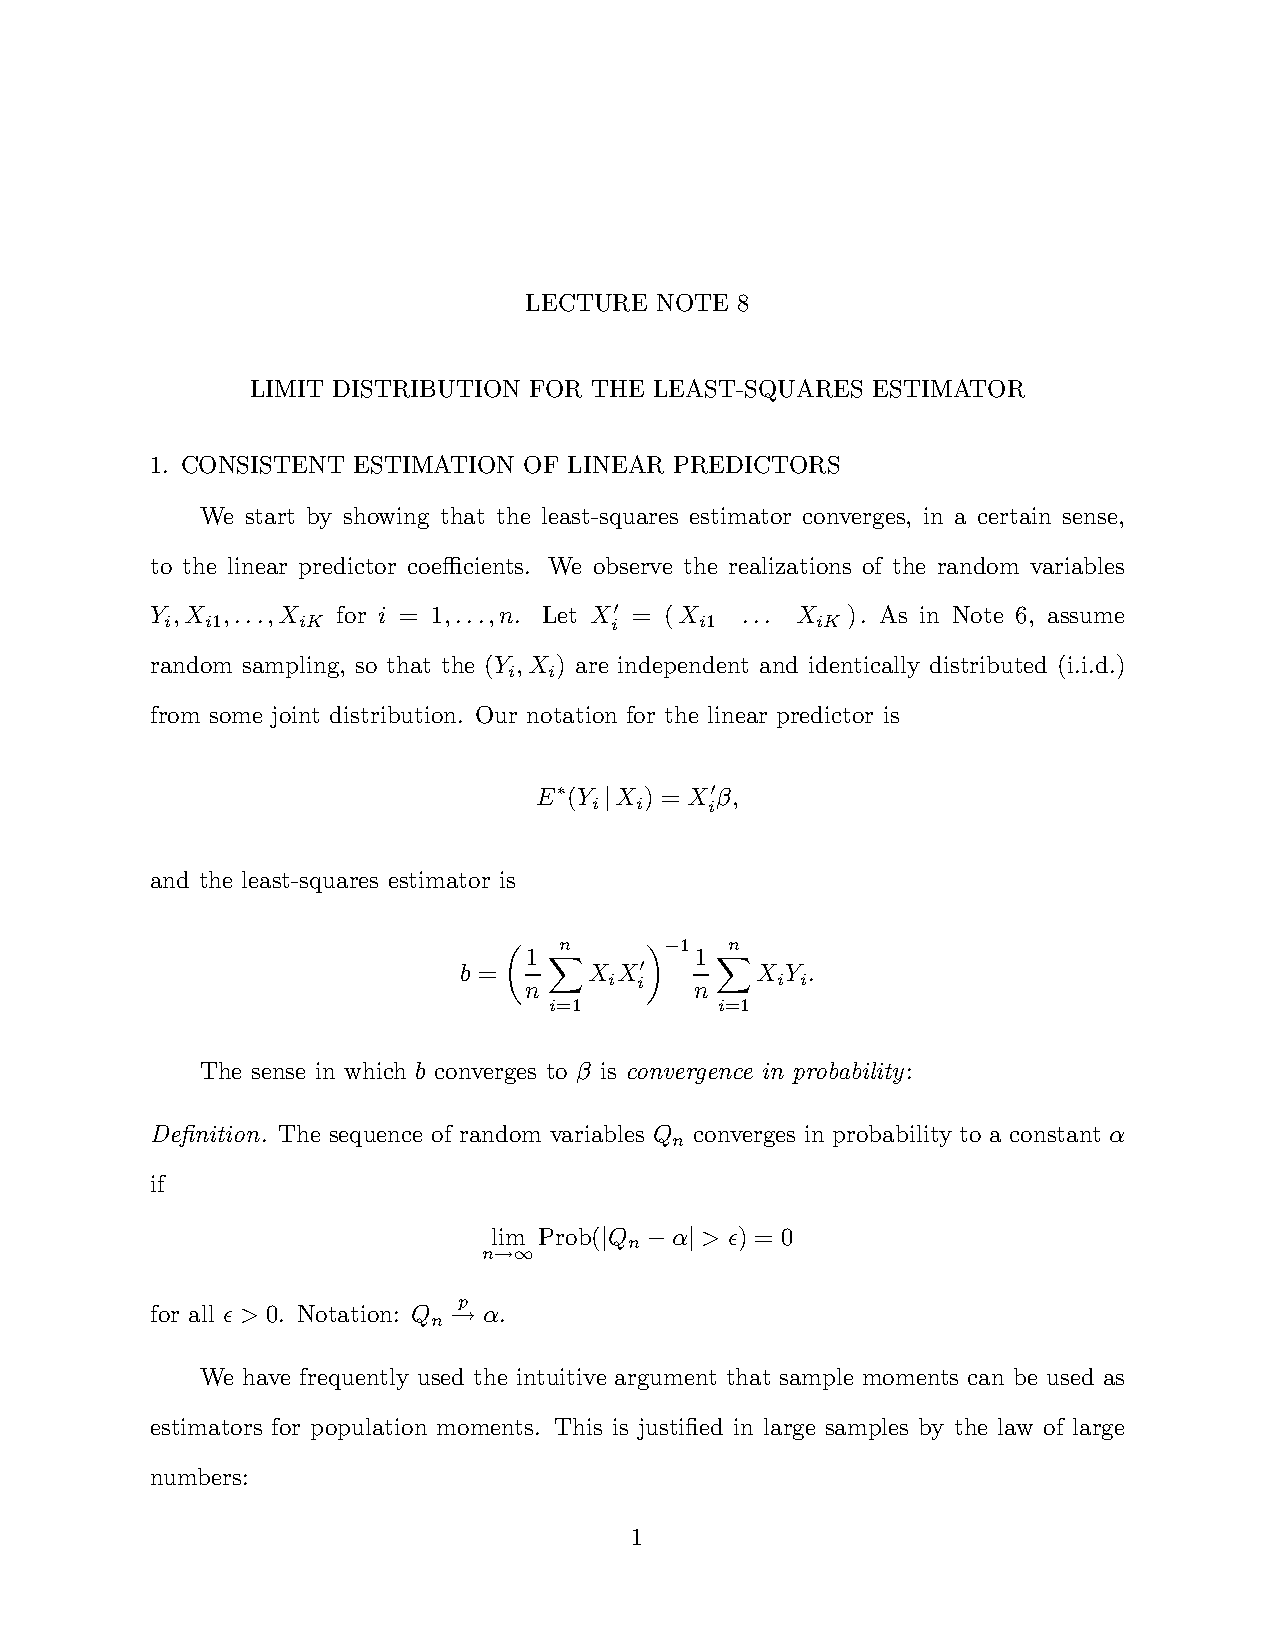
\includepdf[pages=1, pagecommand={\fakesection{Limit Distribution for the Least-Squares Estimator}\label{lecture8}},linktodoc=true,clip,trim=0mm 22mm 0mm 24mm]{Lecture_Note_8.pdf}
\includepdf[pages=2-,pagecommand={},clip,trim=0mm 22mm 0mm 24mm]{Lecture_Note_8.pdf}
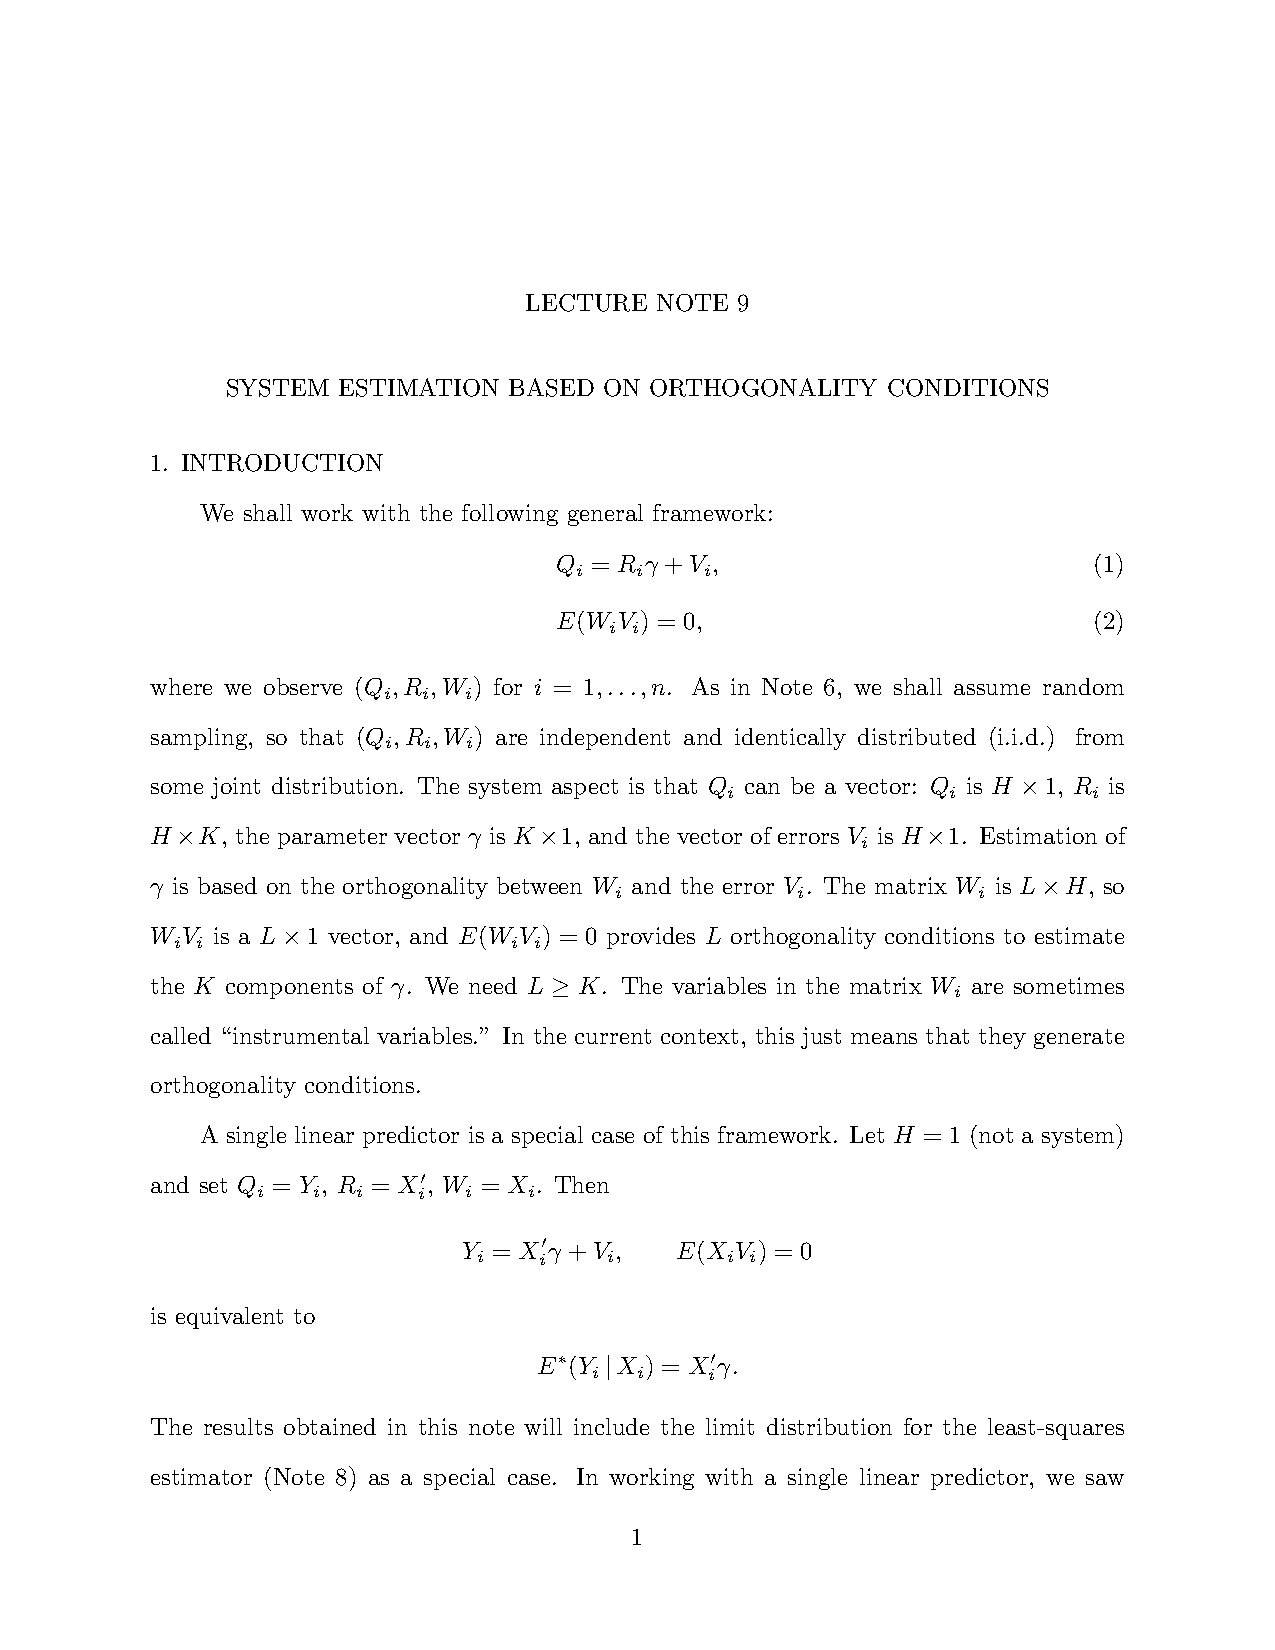
\includepdf[pages=1, pagecommand={\fakesection{System Estimation based on Orthogonality Conditions}\label{lecture9}},linktodoc=true,clip,trim=0mm 22mm 0mm 24mm]{Lecture_Note_9.pdf}
\includepdf[pages=2-,pagecommand={},clip,trim=0mm 22mm 0mm 24mm]{Lecture_Note_9.pdf}
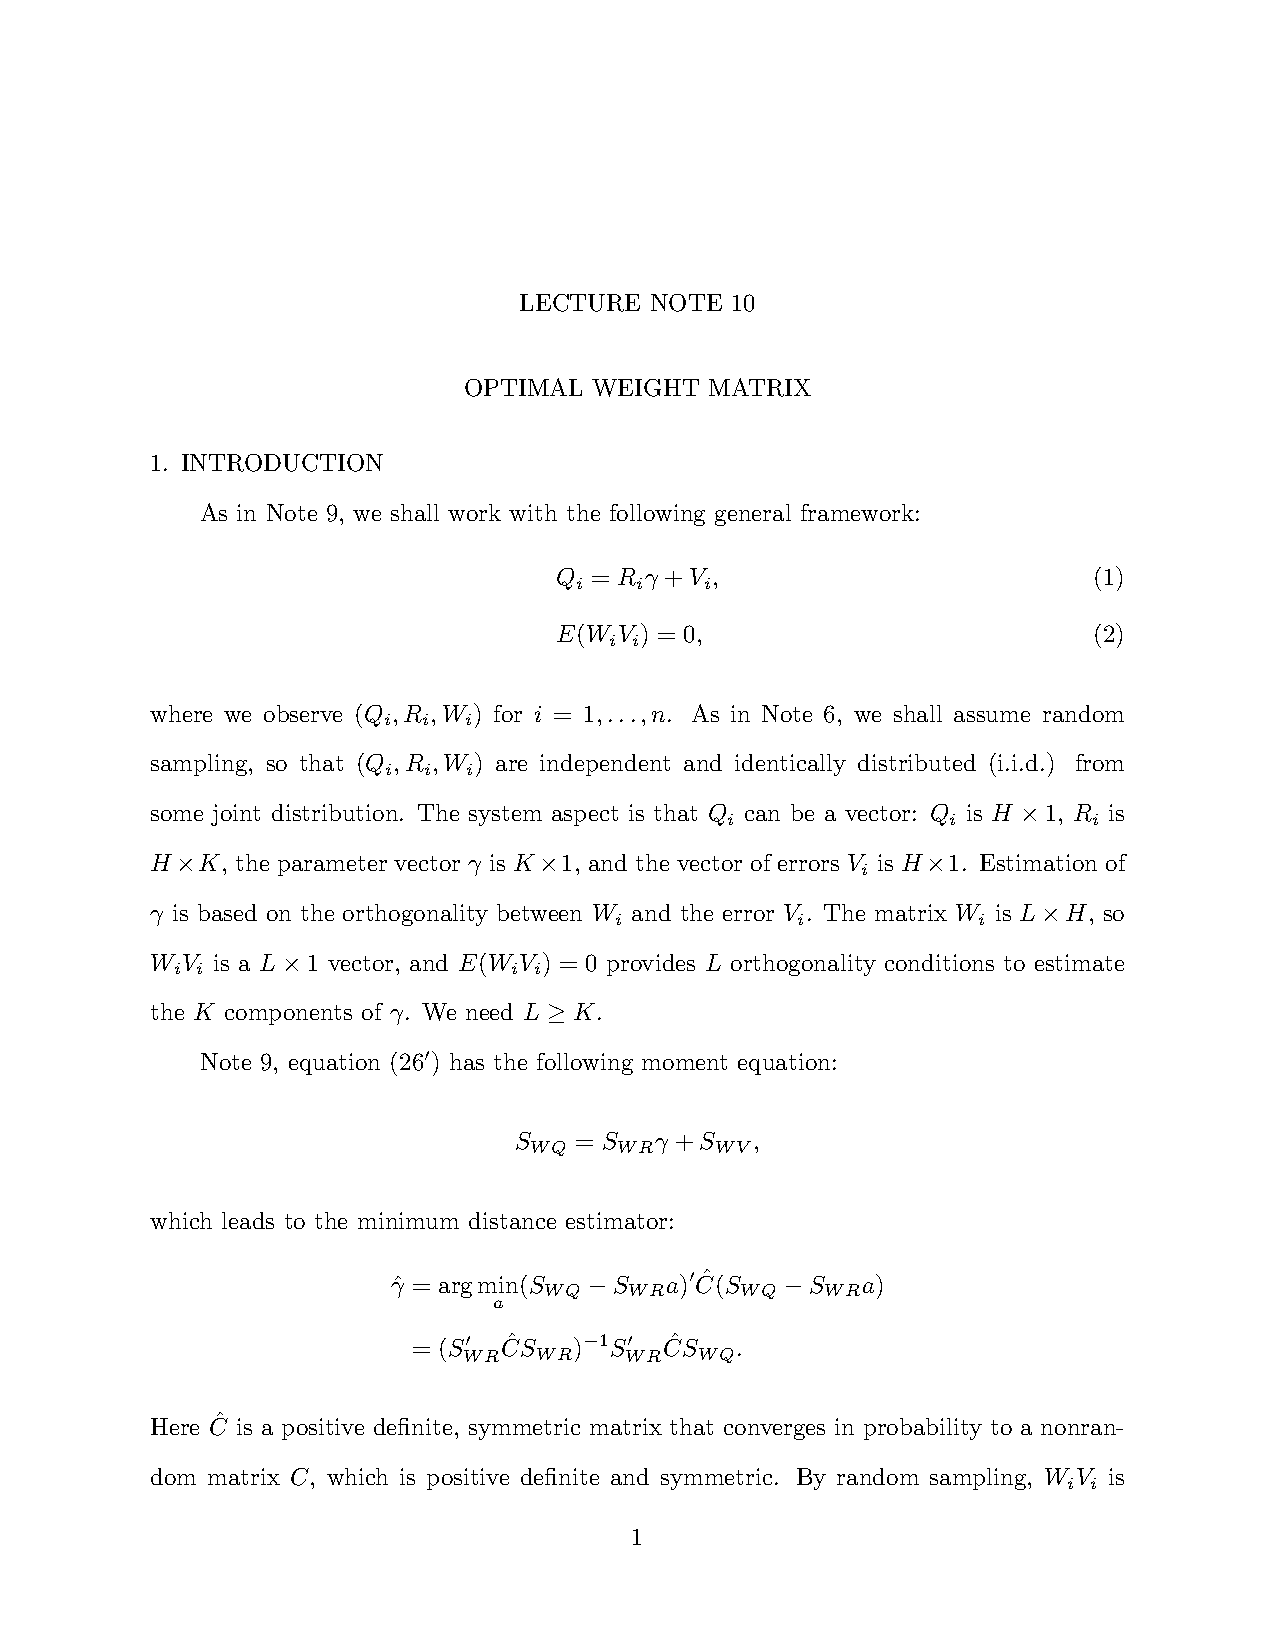
\includepdf[pages=1, pagecommand={\fakesection{Optimal Weight Matrix}\label{lecture10}},linktodoc=true,clip,trim=0mm 22mm 0mm 24mm]{Lecture_Note_10.pdf}
\includepdf[pages=2-,pagecommand={},clip,trim=0mm 22mm 0mm 24mm]{Lecture_Note_10.pdf}
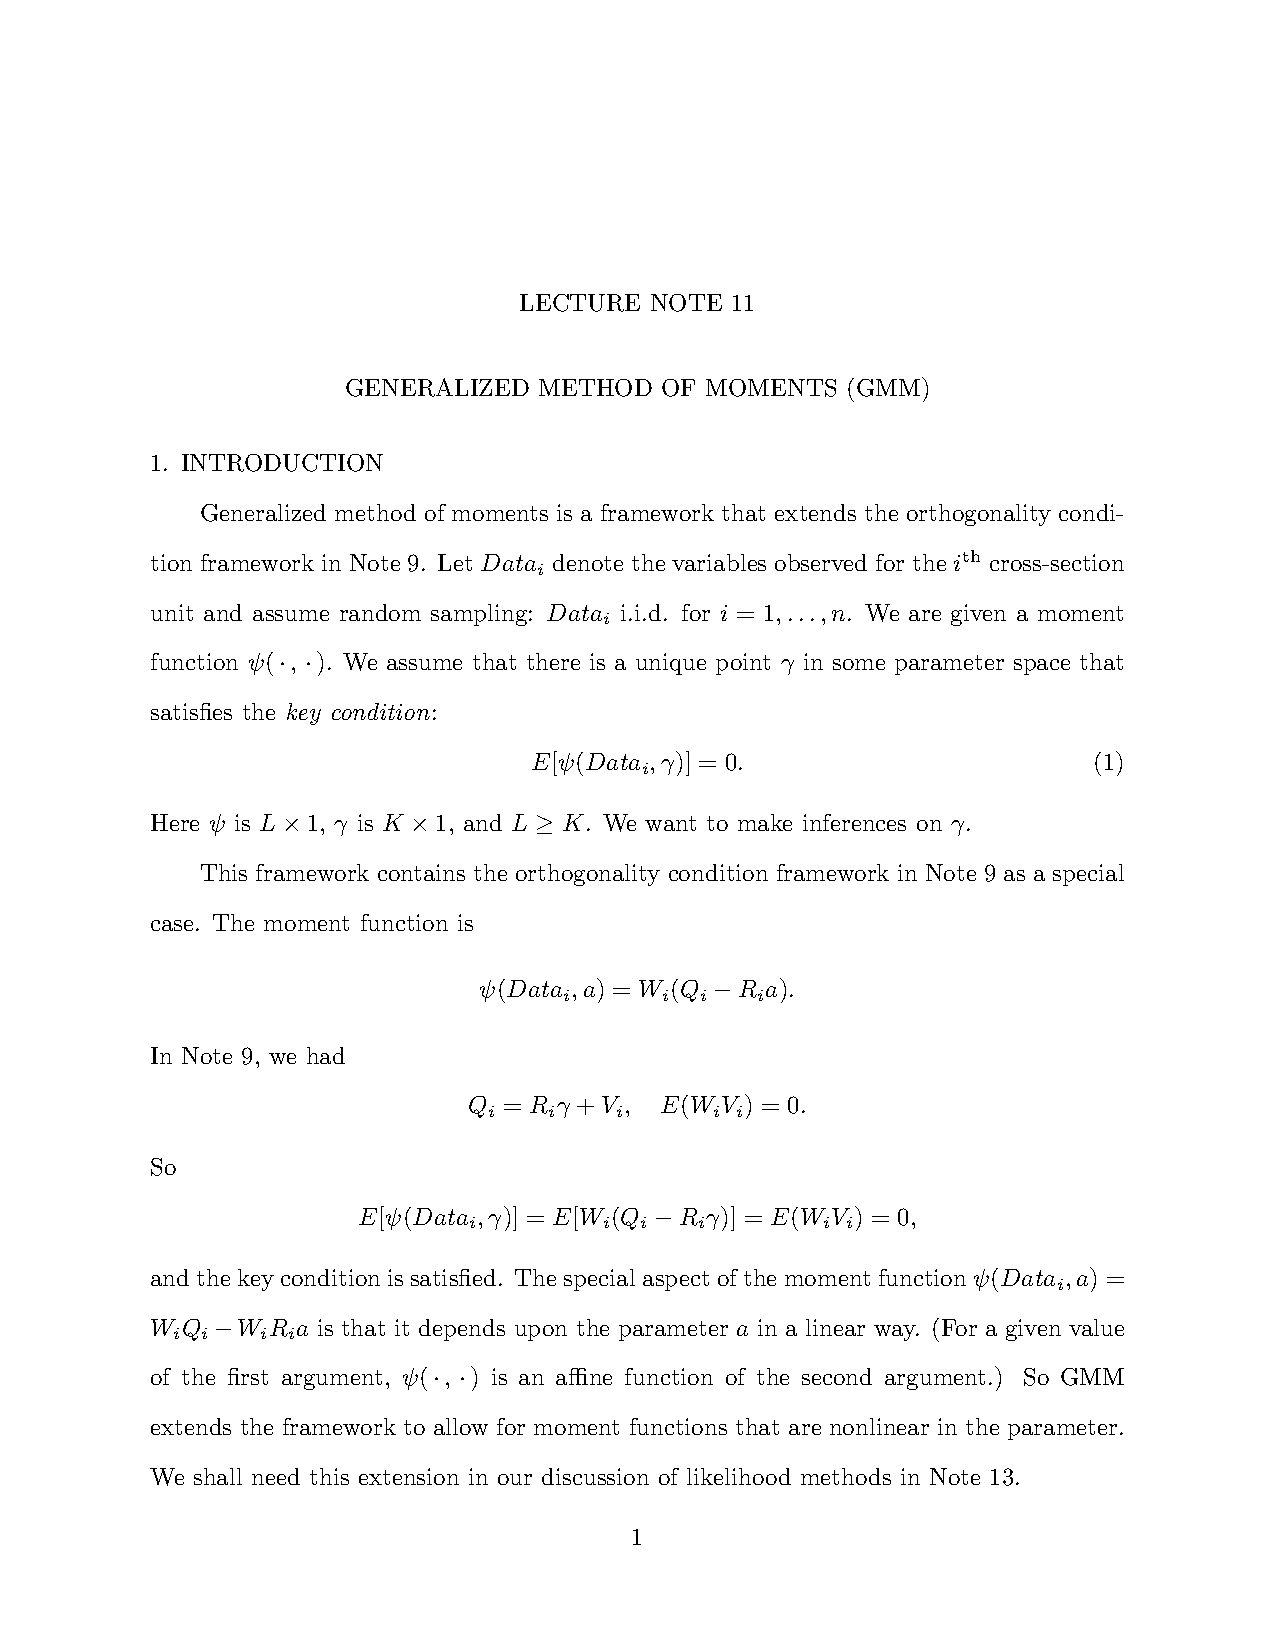
\includepdf[pages=1, pagecommand={\fakesection{Generalized Method of Moments}\label{lecture11}},linktodoc=true,clip,trim=0mm 22mm 0mm 24mm]{Lecture_Note_11.pdf}
\includepdf[pages=2-,pagecommand={},clip,trim=0mm 22mm 0mm 24mm]{Lecture_Note_11.pdf}
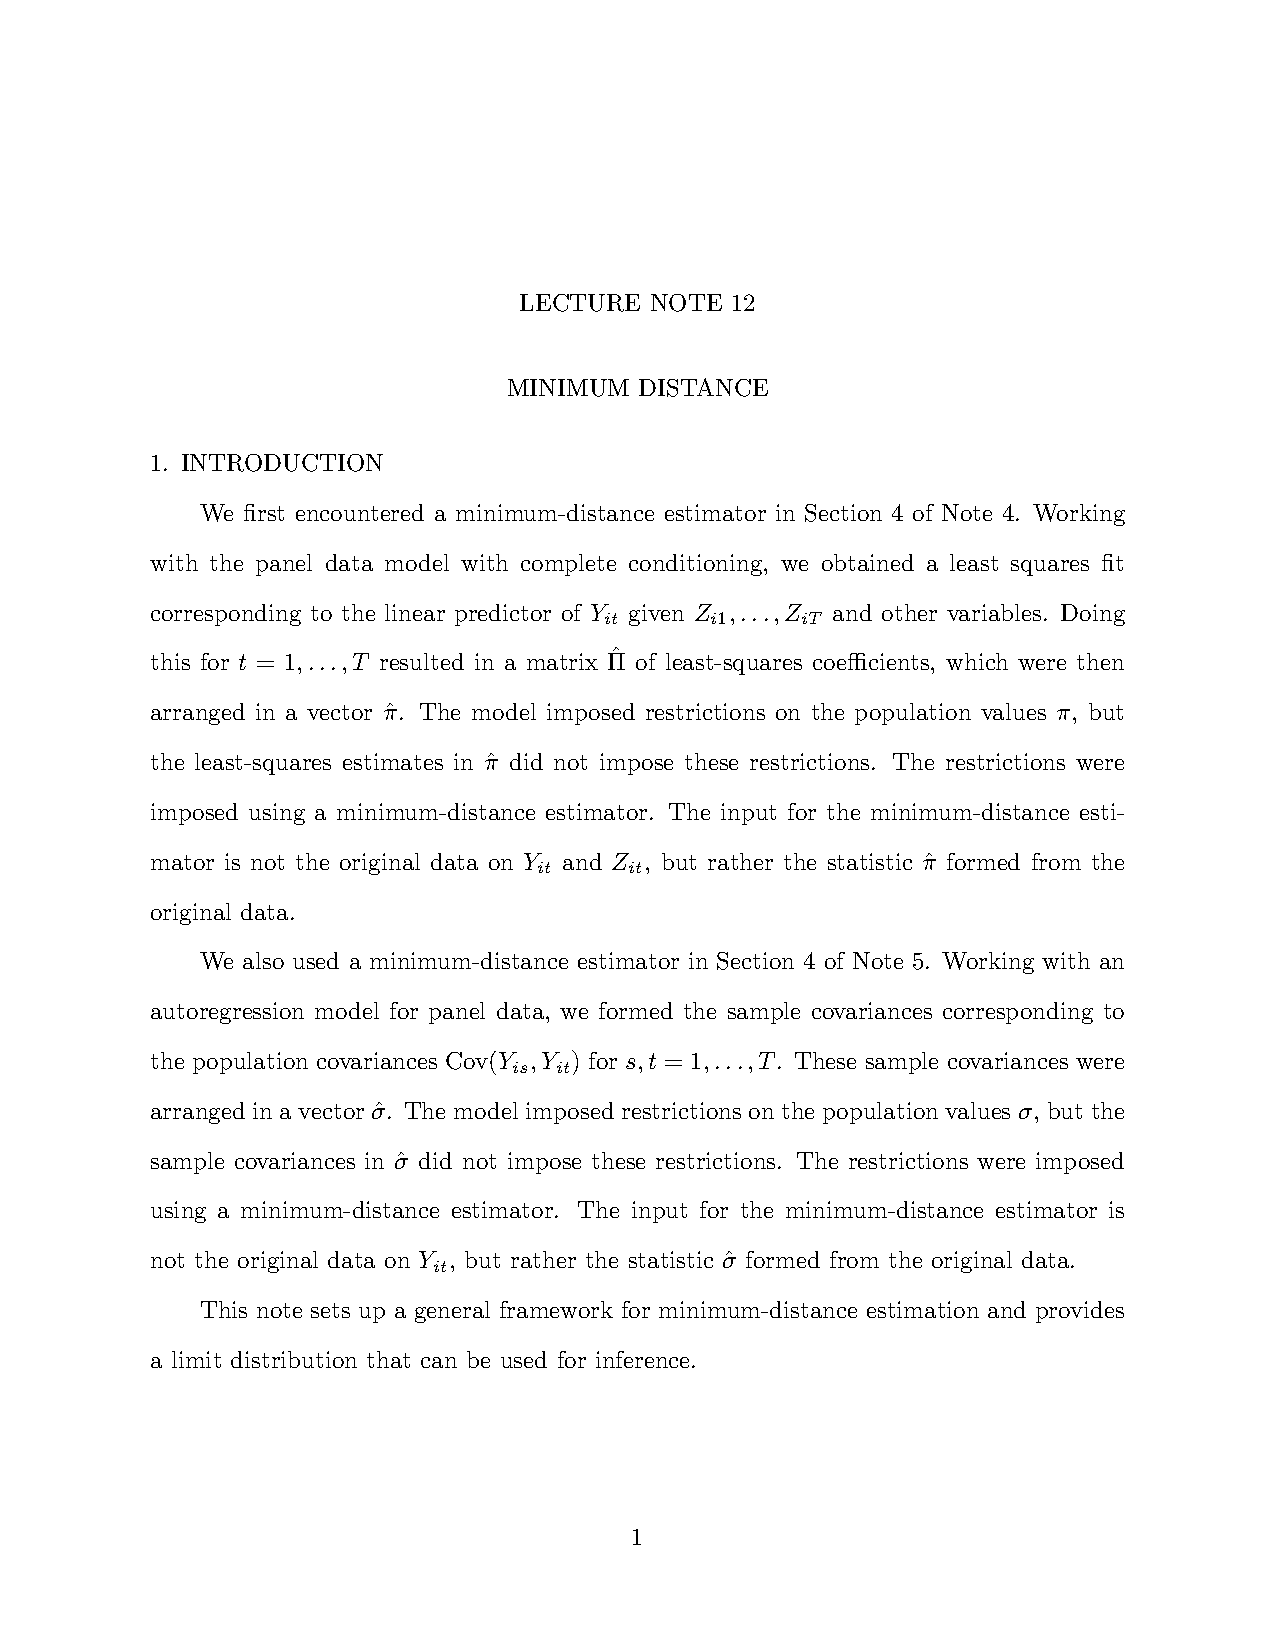
\includepdf[pages=1, pagecommand={\fakesection{Minimum Distance}\label{lecture12}},linktodoc=true,clip,trim=0mm 22mm 0mm 24mm]{Lecture_Note_12.pdf}
\includepdf[pages=2-,pagecommand={},clip,trim=0mm 22mm 0mm 24mm]{Lecture_Note_12.pdf}
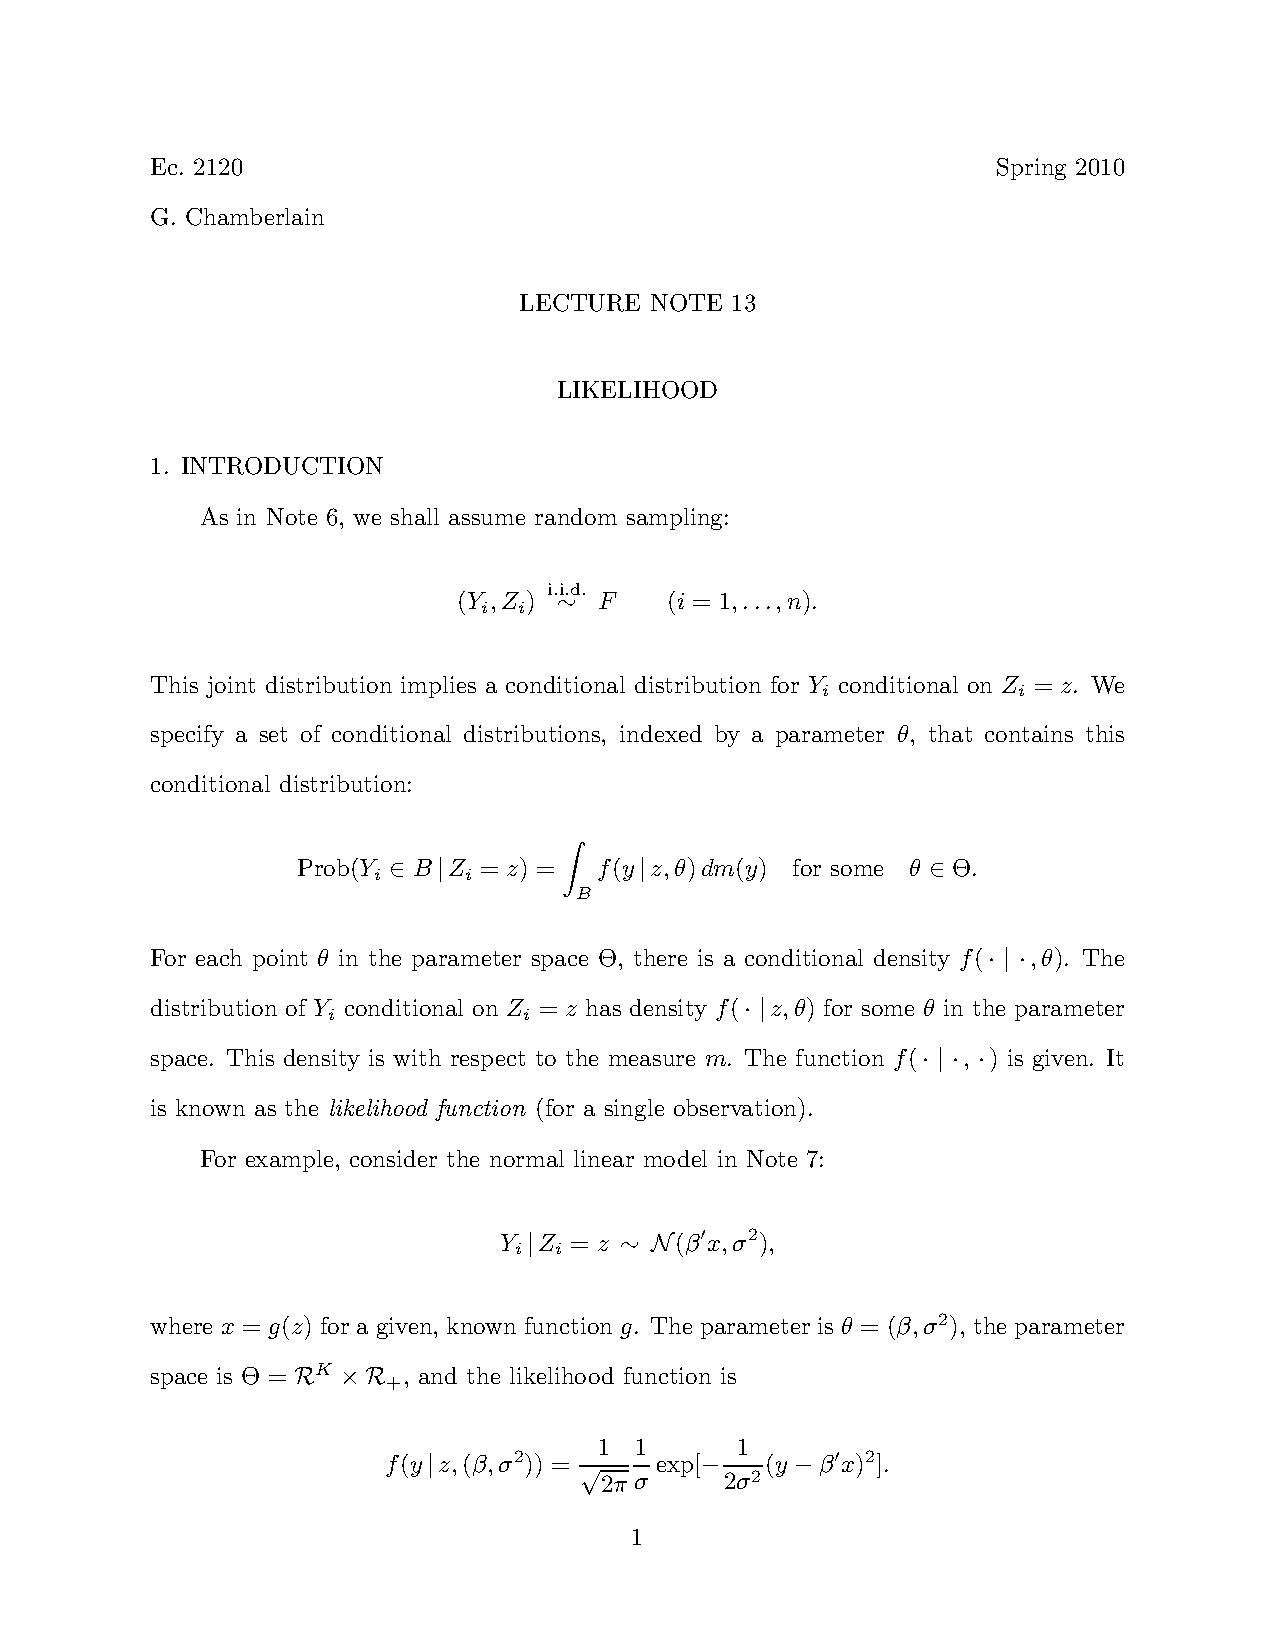
\includepdf[pages=1, pagecommand={\fakesection{Likelihood}\label{lecture13}},linktodoc=true,clip,trim=0mm 22mm 0mm 24mm]{Lecture_Note_13.pdf}
\includepdf[pages=2-,pagecommand={},clip,trim=0mm 22mm 0mm 24mm]{Lecture_Note_13.pdf}
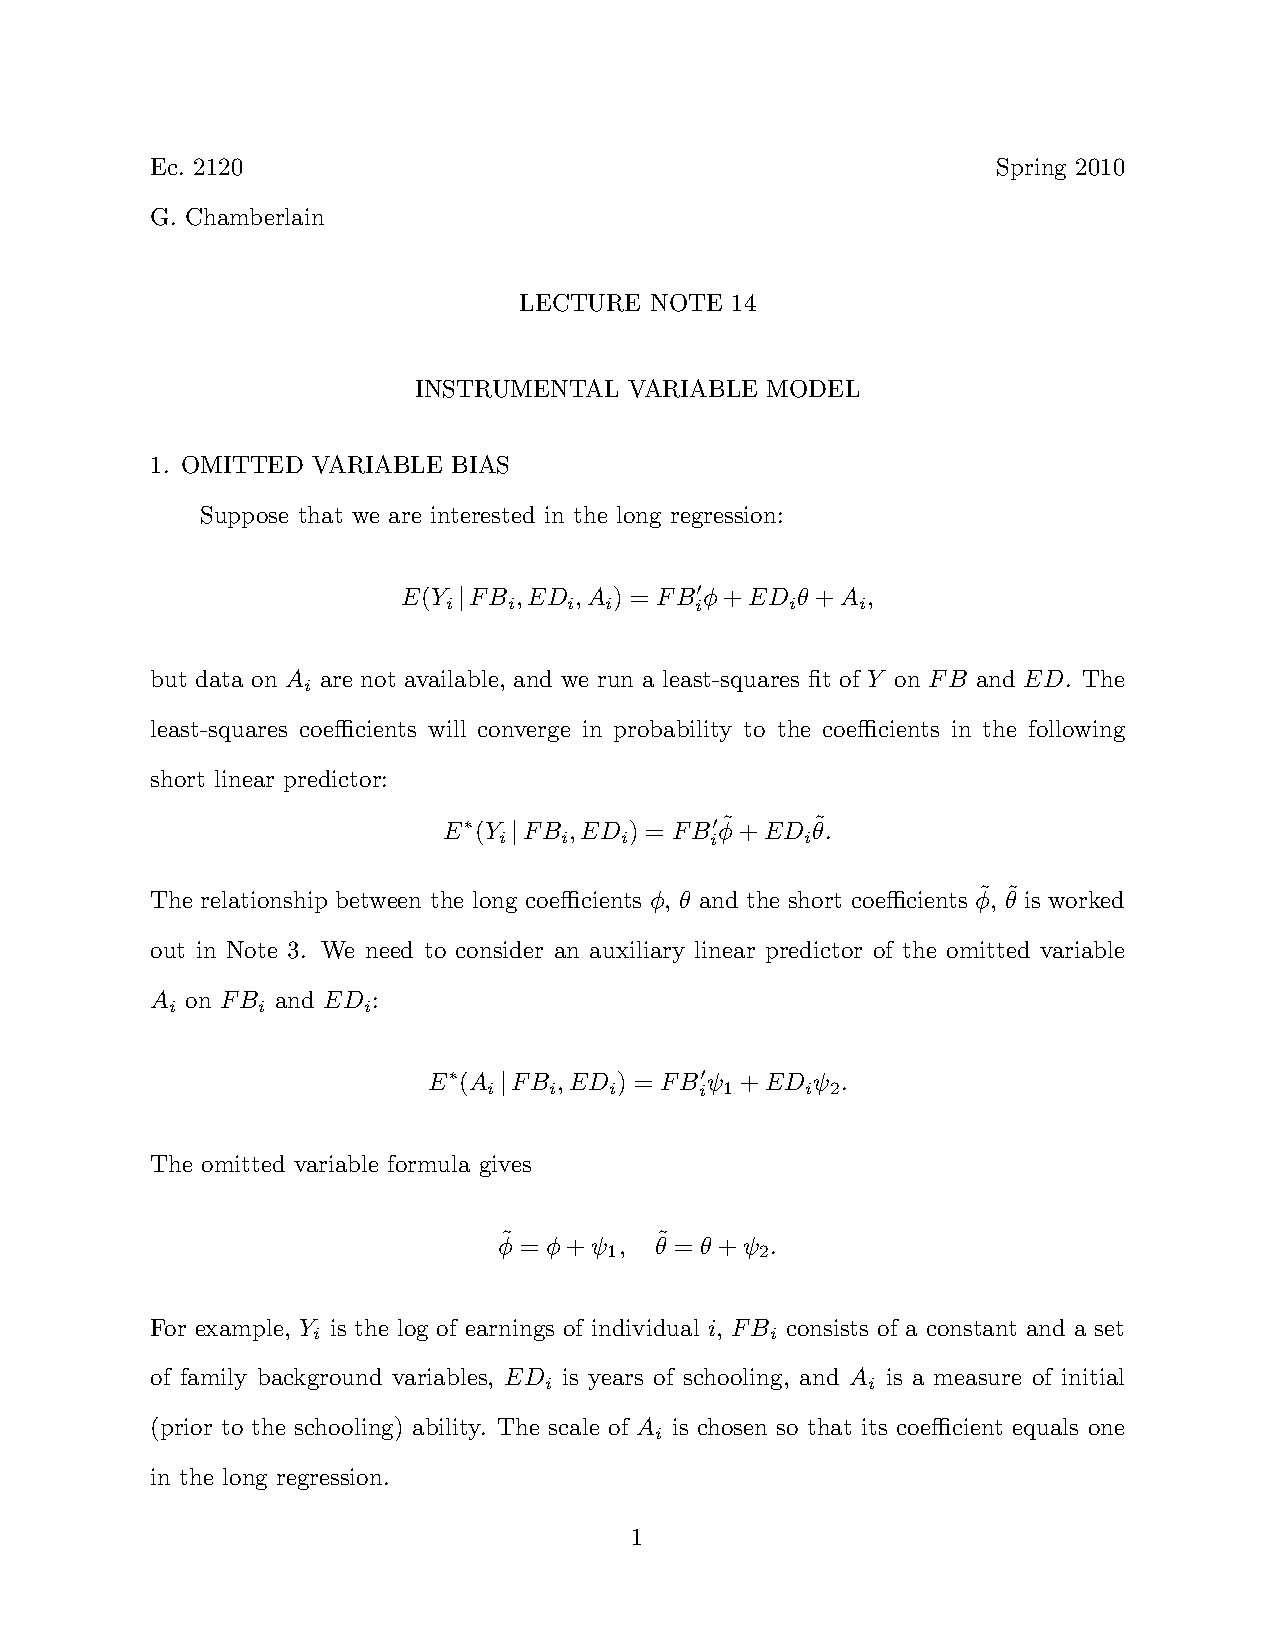
\includepdf[pages=1, pagecommand={\fakesection{Instrumental Variable Model}\label{lecture14}},linktodoc=true,clip,trim=0mm 22mm 0mm 24mm]{Lecture_Note_14.pdf}
\includepdf[pages=2-,pagecommand={},clip,trim=0mm 22mm 0mm 24mm]{Lecture_Note_14.pdf}
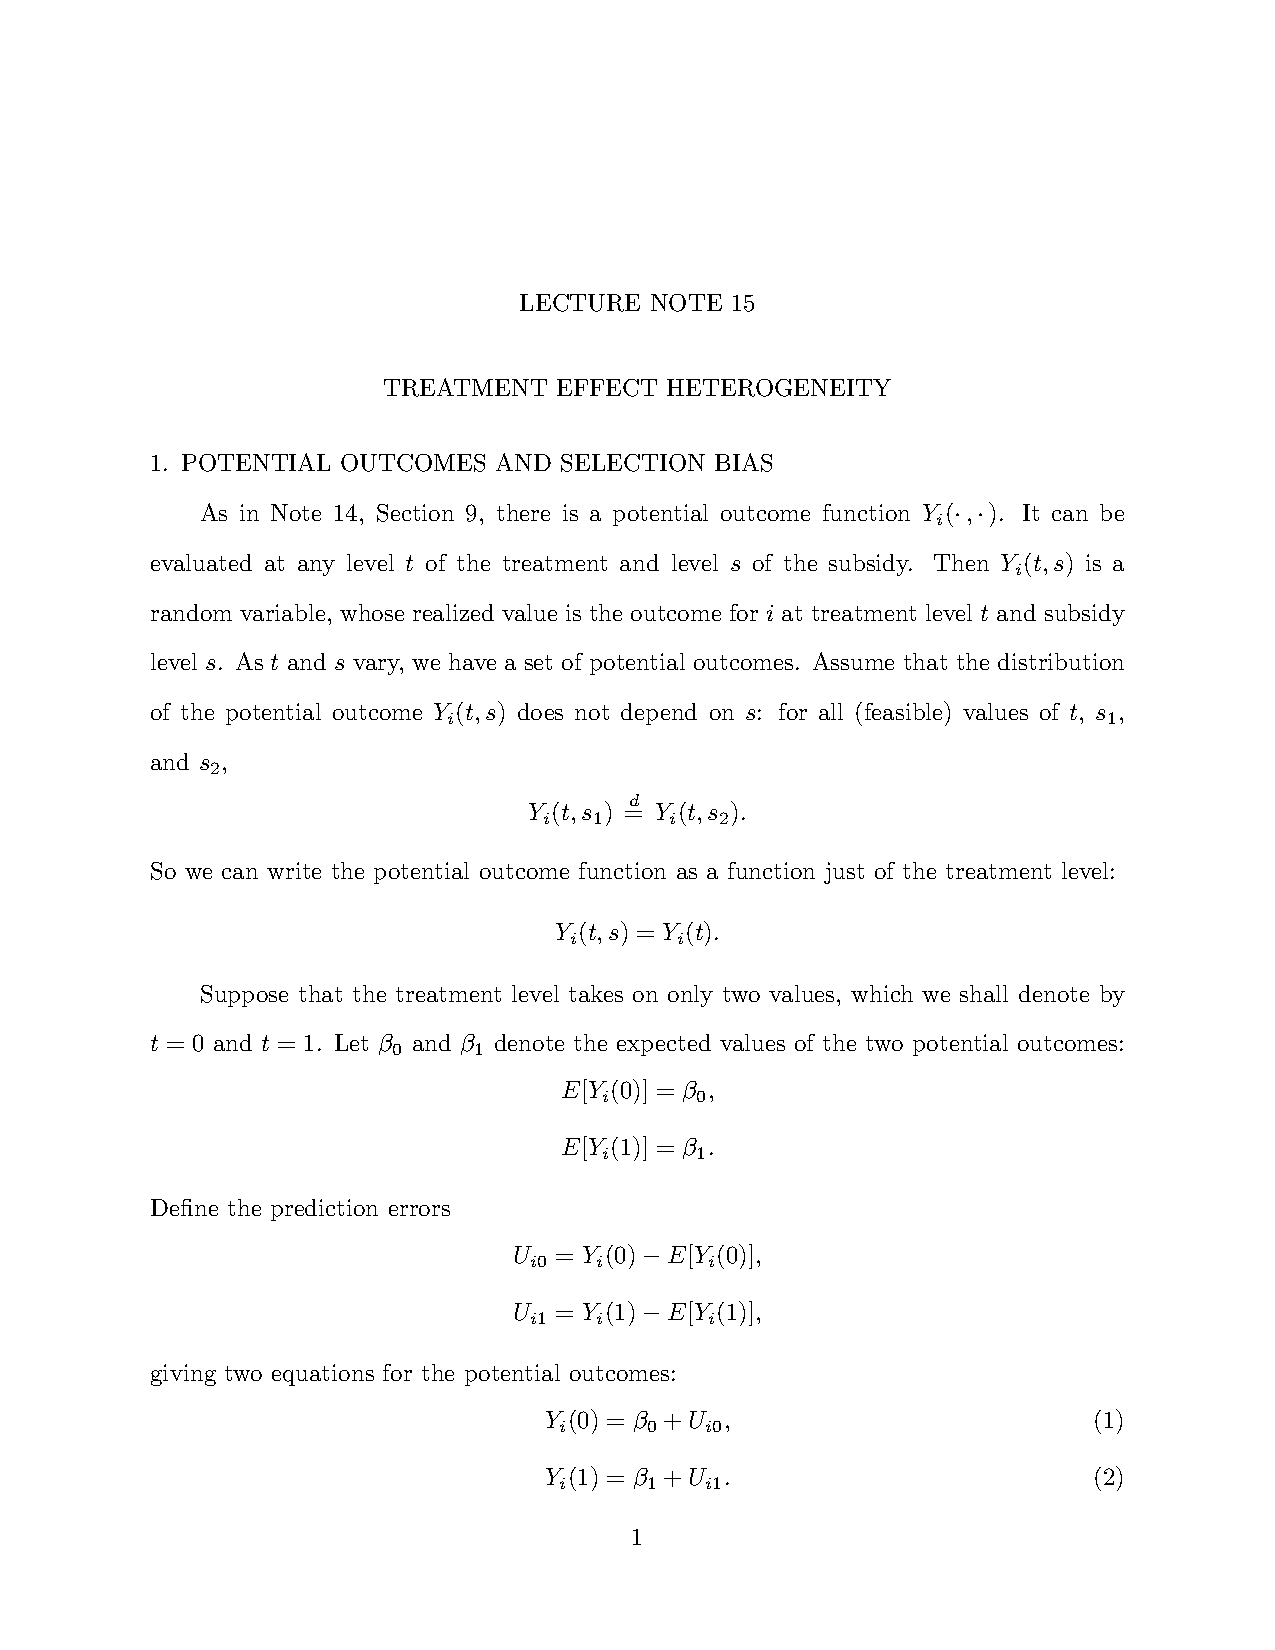
\includepdf[pages=1, pagecommand={\fakesection{Treatment Effect Heterogeneity}\label{lecture15}},linktodoc=true,clip,trim=0mm 22mm 0mm 24mm]{Lecture_Note_15.pdf}
\includepdf[pages=2-,pagecommand={},clip,trim=0mm 22mm 0mm 24mm]{Lecture_Note_15.pdf}
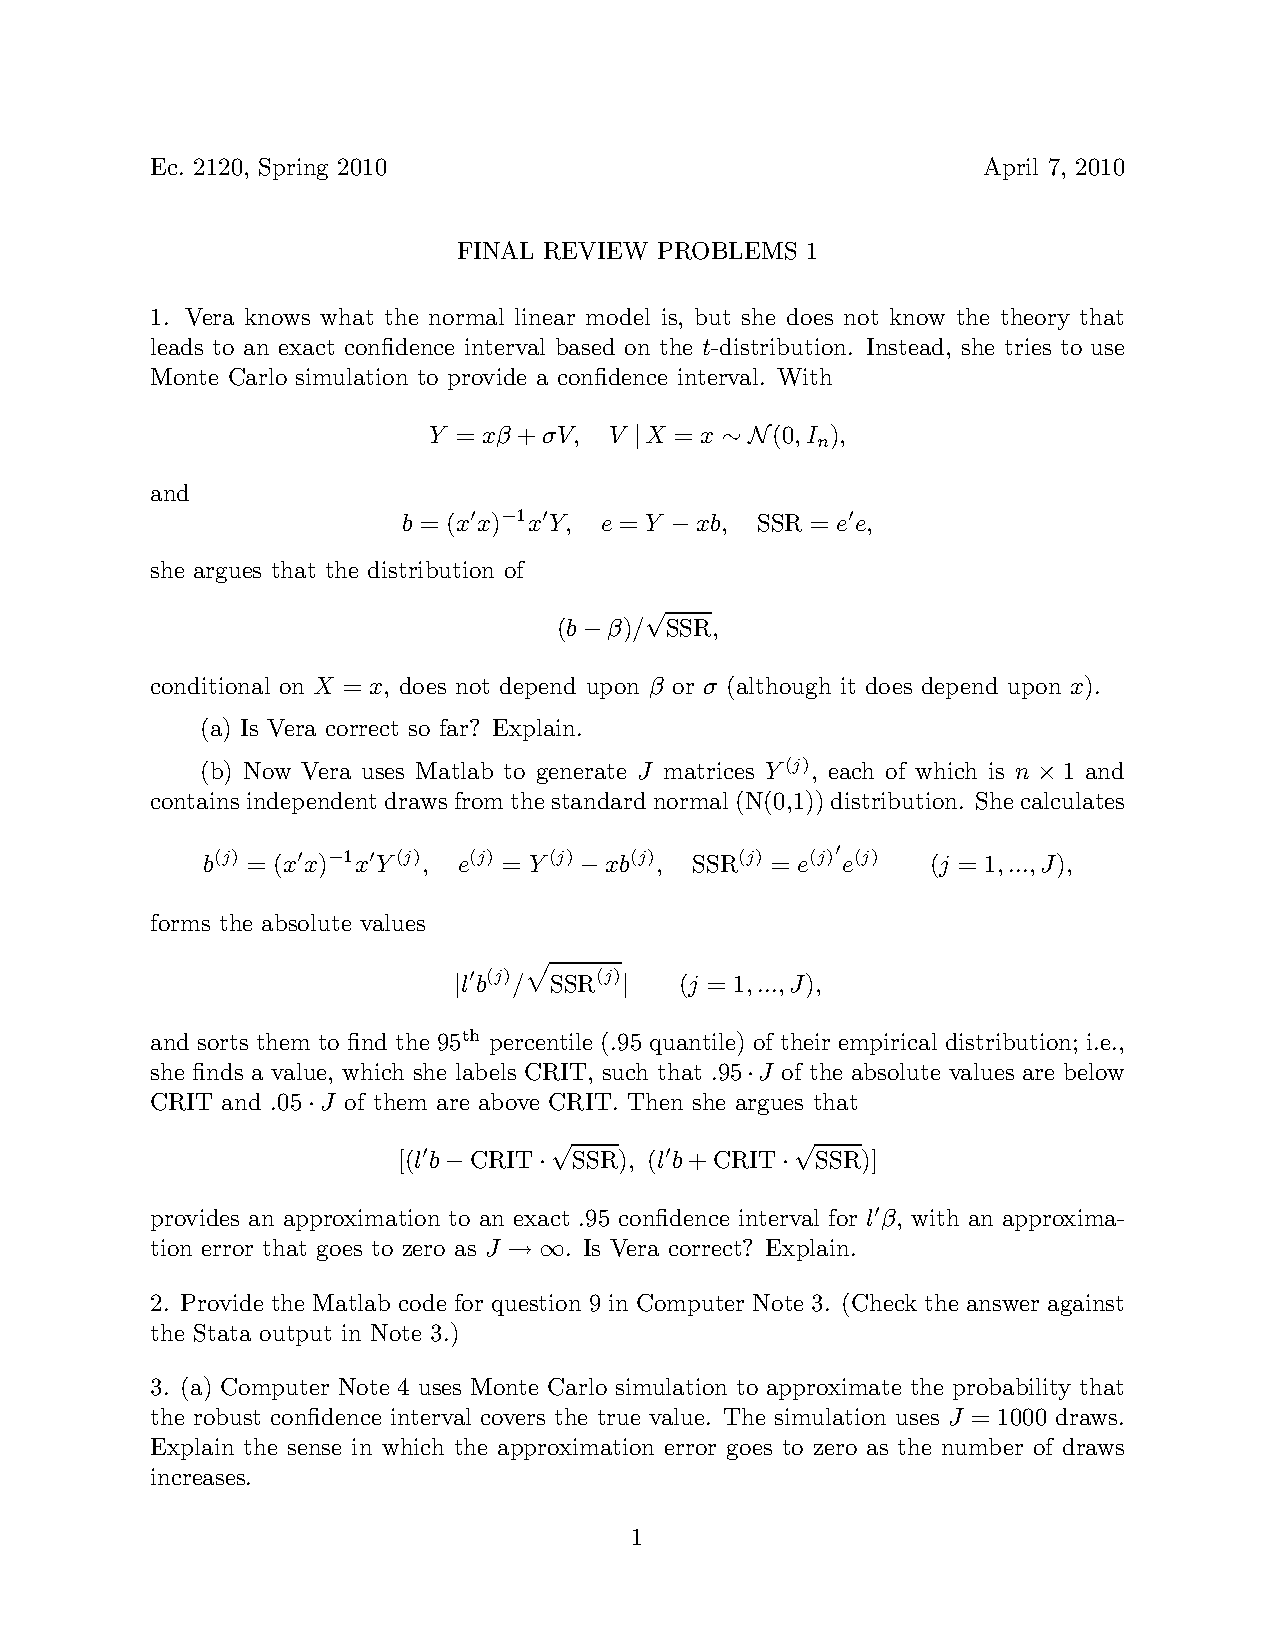
\includepdf[pages=1, pagecommand={\fakesectionb{Review Problems 1}\label{reviewproblems}},linktodoc=true,clip,trim=0mm 22mm 0mm 24mm]{Final_Review_Problems_1.pdf}
\includepdf[pages=2-,pagecommand={},clip,trim=0mm 22mm 0mm 24mm]{Final_Review_Problems_1.pdf}
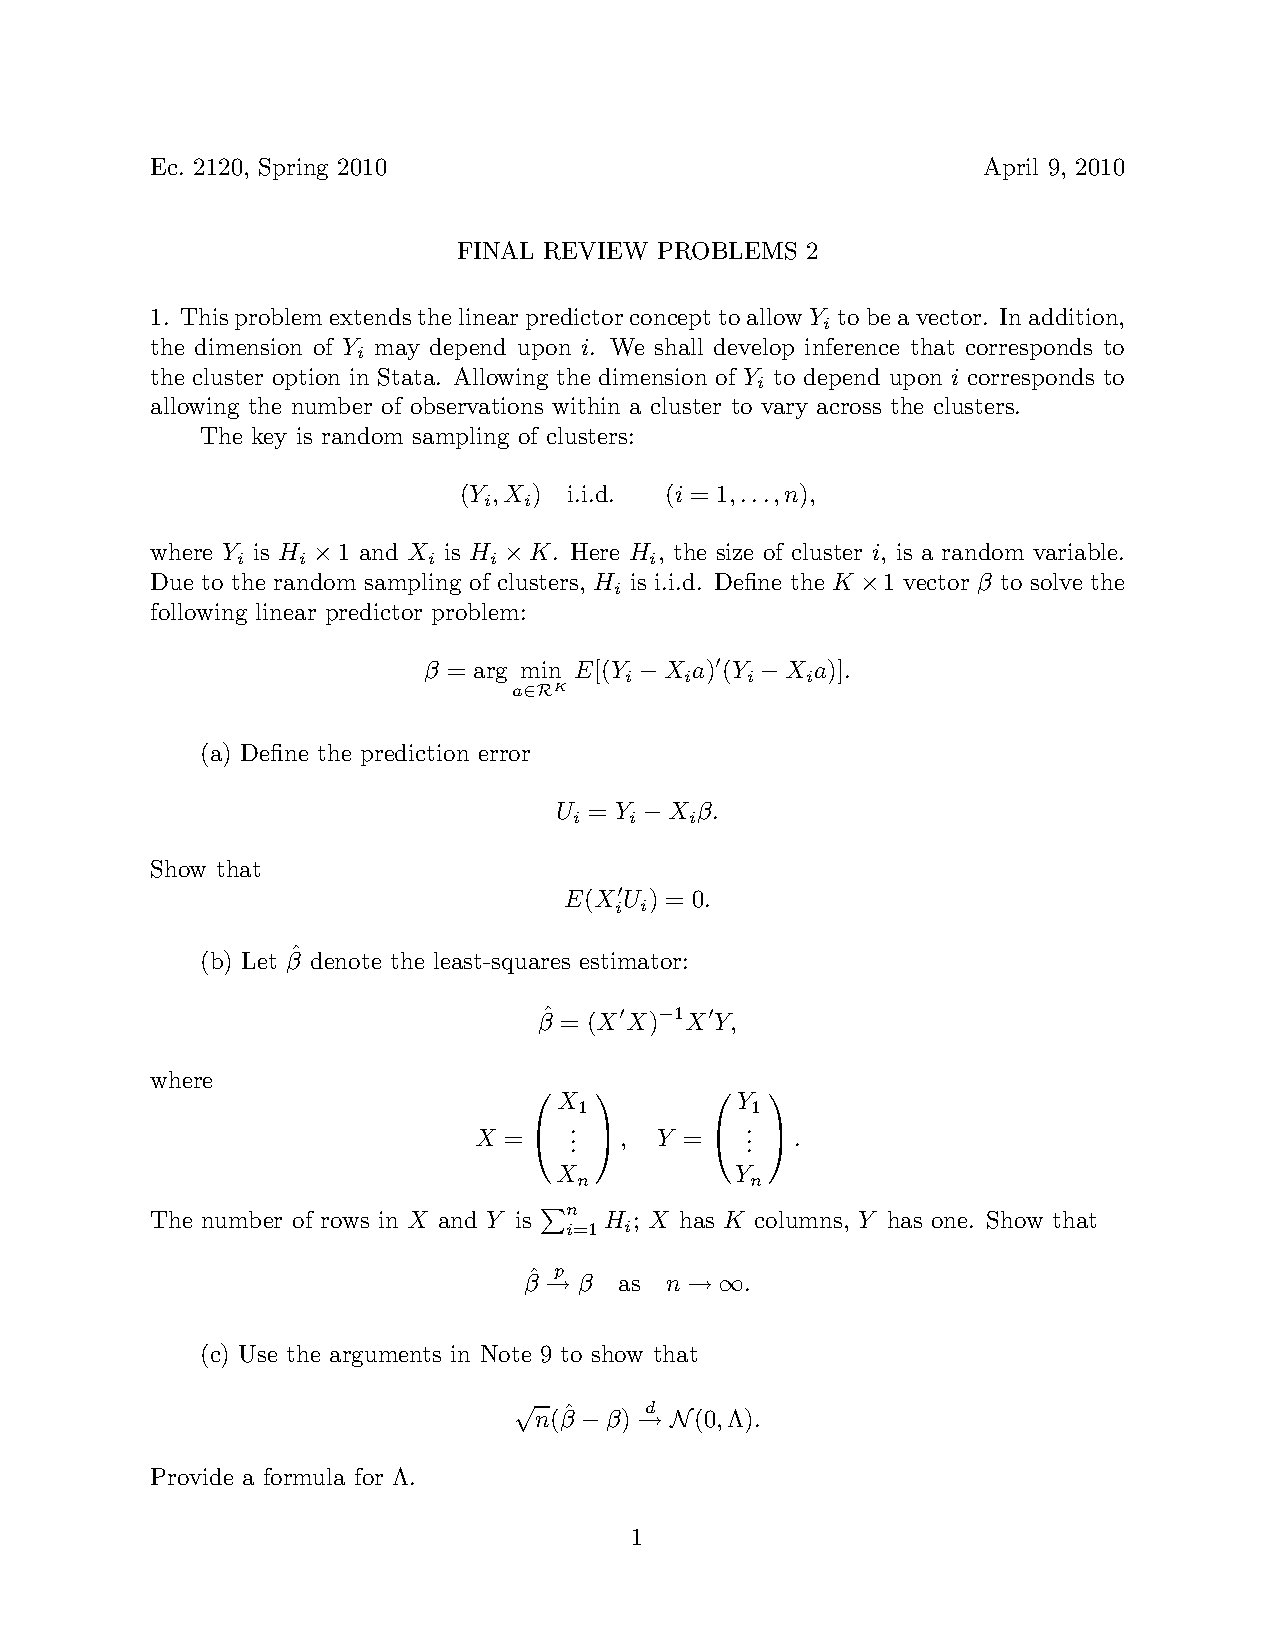
\includepdf[pages=1, pagecommand={\fakesectionb{Review Problems 2}\label{reviewproblems2}},linktodoc=true,clip,trim=0mm 22mm 0mm 24mm]{Final_Review_Problems_2.pdf}
\includepdf[pages=2-,pagecommand={},clip,trim=0mm 22mm 0mm 24mm]{Final_Review_Problems_2.pdf}
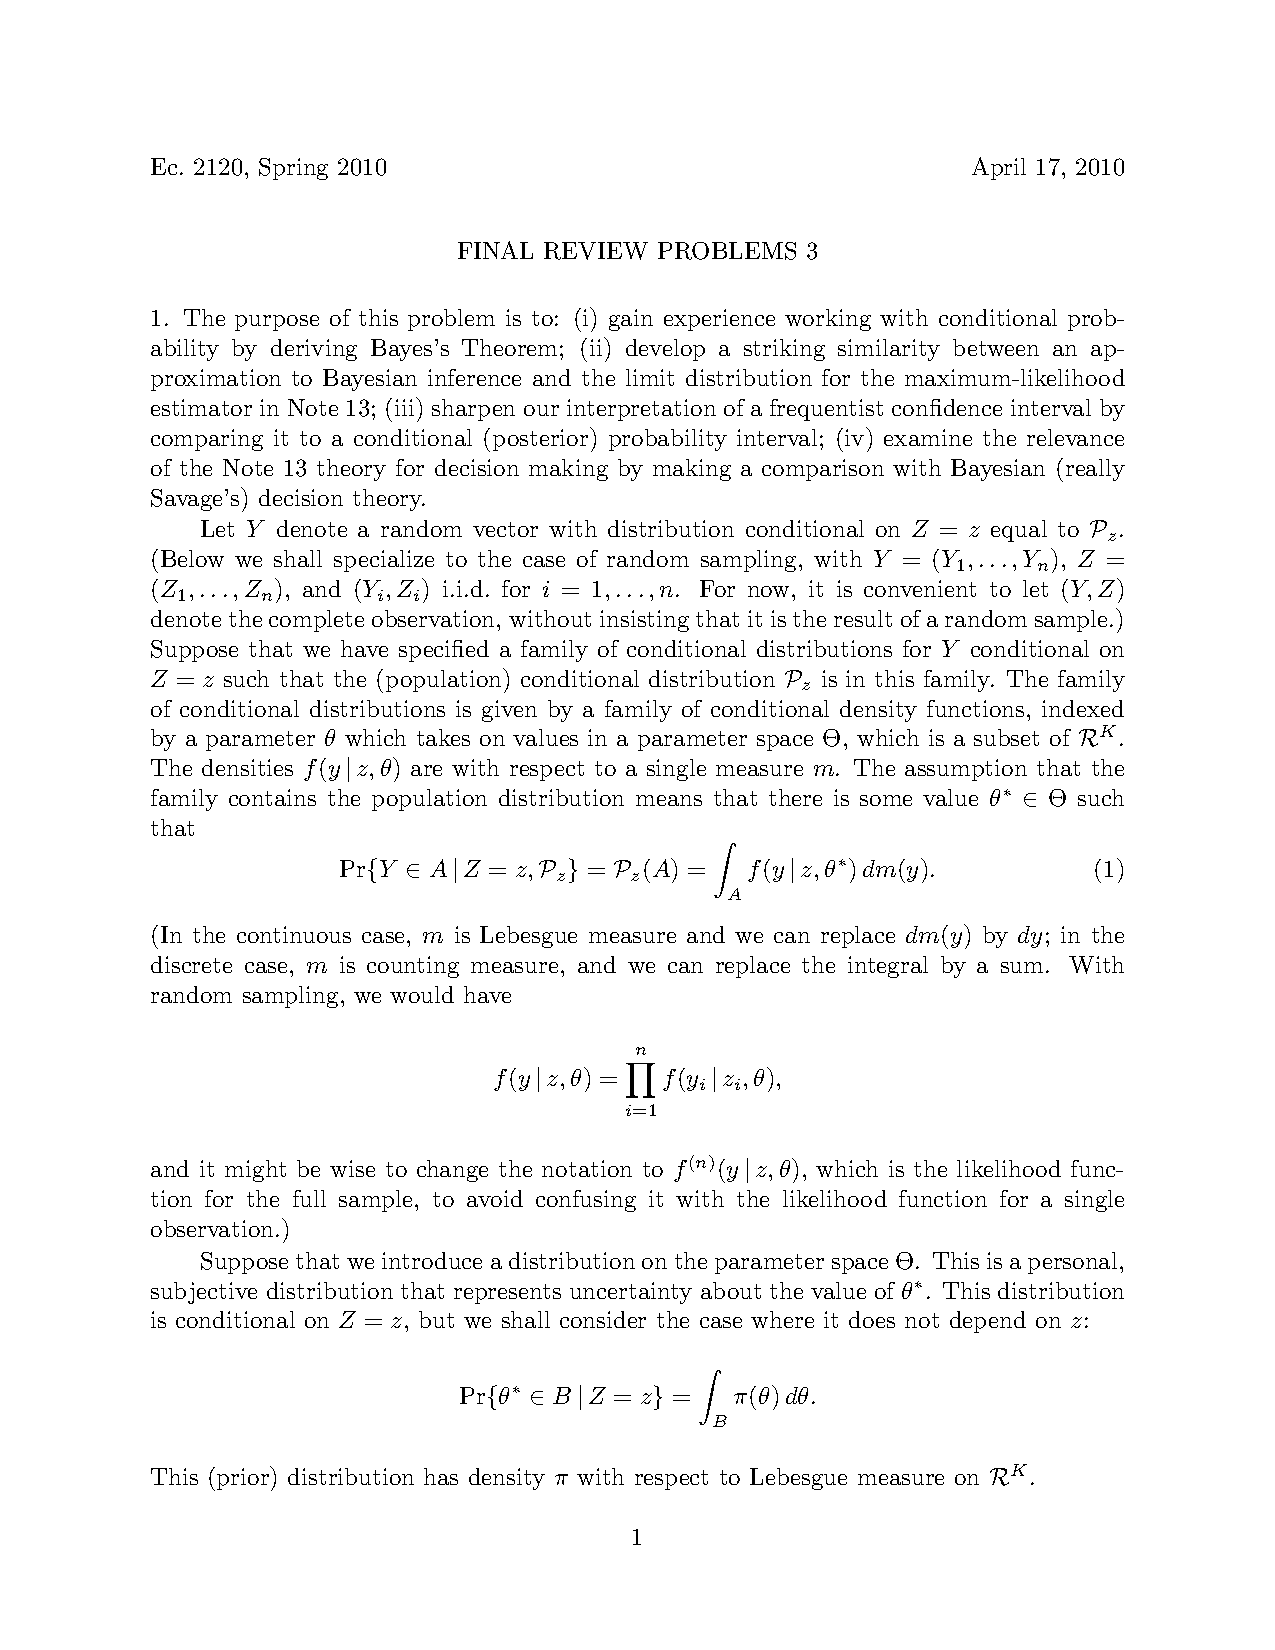
\includepdf[pages=1, pagecommand={\fakesectionb{Review Problems 3}\label{reviewproblems3}},linktodoc=true,clip,trim=0mm 22mm 0mm 24mm]{Final_Review_Problems_3.pdf}
\includepdf[pages=2-,pagecommand={},clip,trim=0mm 22mm 0mm 24mm]{Final_Review_Problems_3.pdf}
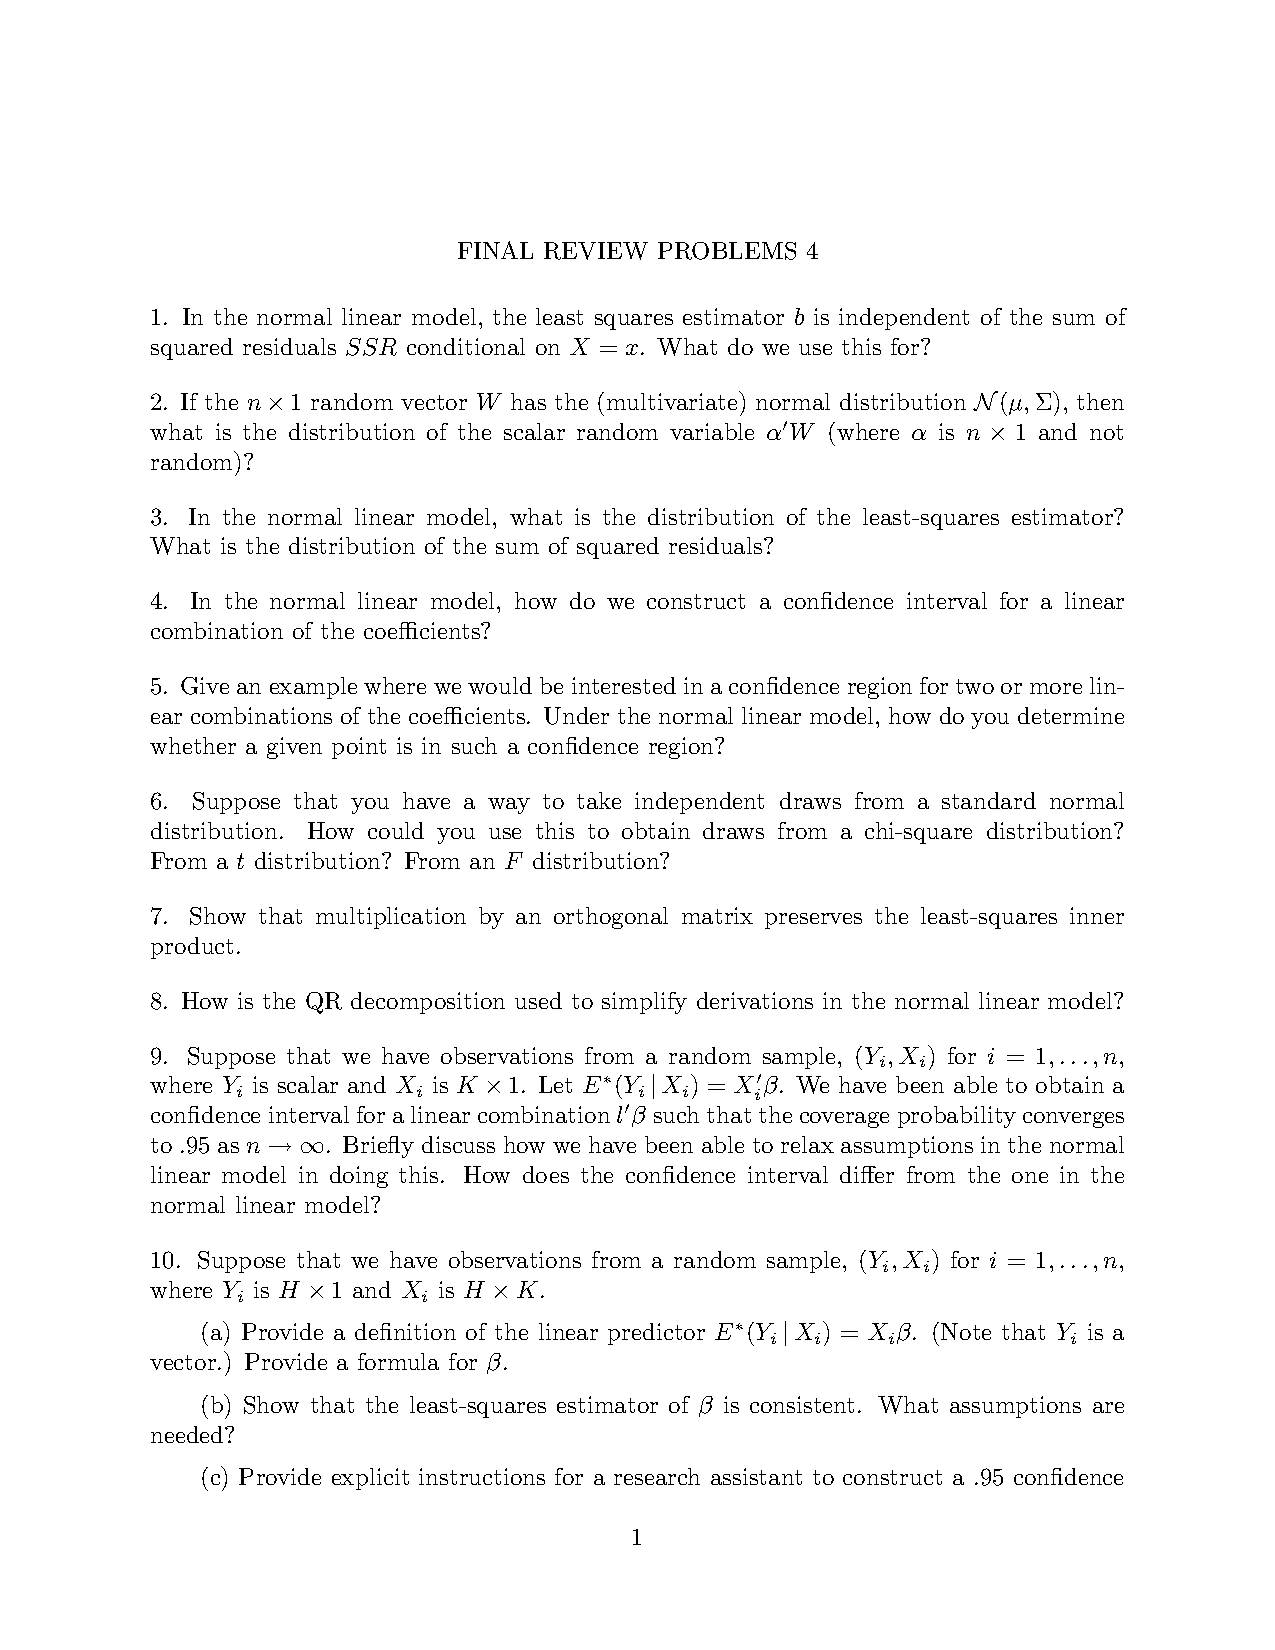
\includepdf[pages=1, pagecommand={\fakesectionb{Review Problems 4}\label{reviewproblems4}},linktodoc=true,clip,trim=0mm 22mm 0mm 24mm]{Final_Review_Problems_4.pdf}
\includepdf[pages=2-,pagecommand={},clip,trim=0mm 22mm 0mm 24mm]{Final_Review_Problems_4.pdf}


\end{document}